\documentclass{article}
\usepackage[margin=1in,footskip=0.25in]{geometry}
\usepackage{graphicx}
\usepackage{lipsum} 
\usepackage{fullpage}
\setlength{\textwidth}{6.5in}
\setlength{\oddsidemargin}{.1in}
\setlength{\evensidemargin}{.1in}
\setlength{\topmargin}{-.1in}
\setlength{\textheight}{8.4in}


\usepackage[colorlinks=true,
linkcolor=blue,
filecolor=blue,
citecolor=blue]{hyperref}
\usepackage{titling}
\usepackage{amsmath} 
\usepackage{amssymb}
\usepackage{array}
\usepackage{mdframed}
\usepackage{yhmath}
\usepackage{tikz}
\usepackage{tikz-3dplot}
\usetikzlibrary{decorations.markings,3d,shadings, backgrounds, positioning}
\usepackage{blochsphere}


\tikzset{->-/.style={decoration={markings, mark=at position #1 with {\arrow{>}}}, postaction={decorate}}, ->-/.default=0.5}


\title{\textbf{The Generalised Stokes Theorem and Calculus on Manifolds}}
\author{Vishnu Varadarajan
\\
Ashoka University, Sonipat\\
\href{mailto:vishnu.varadarajan\_ug2023@ashoka.edu.in}{\tt vishnu.varadarajan\_ug2023@ashoka.edu.in}}
\date{\today}
\newcounter{definition}[section]
\renewcommand{\thedefinition}{\thesection.\arabic{definition}}


\newcommand{\rotparl}{\mathbin{\rotatebox[origin=c]{90}{$($}}}
\newcommand{\rotparr}{\mathbin{\rotatebox[origin=c]{90}{$)$}}}
\newcommand{\rotin}{\mathbin{\rotatebox[origin=c]{90}{$\in$}}}
% Define a new environment for definitions
\newenvironment{definition}[1] % #1 is the title of the definition
{%
    \refstepcounter{definition}%
    \noindent\textbf{Definition \thedefinition:} {\textit{#1}}\par\nobreak\noindent
    \begin{quote}
}%
{%
    \end{quote}
}

\newenvironment{theorem}[1] % #1 is the title of the definition
{%
    \refstepcounter{definition}%
    \noindent\textbf{Theorem \thedefinition:} {\textit{#1}}\par\nobreak\noindent
    \begin{quote} % Adjust the space value to set the tab indent size
}%
{%
    \end{quote}
}

\newenvironment{proposition} % #1 is the title of the definition
{%
    \refstepcounter{definition}%
    \noindent\textbf{Proposition \thedefinition:} \nobreak\noindent
}

\def\endproofmark{$\Box$}
\newenvironment{proof}{\par\noindent{\bf Proof}:}{\endproofmark\smallskip}

\begin{document}

\maketitle

\begin{abstract}
This paper is an exposition of the Generalised Stokes Theorem and covers topics of calculus on manifolds. This study happened in the late 19th and early 20th century after the development of single variate and multivariate calculus. With an introduction to an abstraction of surfaces, in the form of manifolds, came the need for a calculus on it. The paper starts at the ground by defining manifolds and extending ideas of smoothness, boundaries, and orientation to them. It introduces multilinear functions and their algebra, followed by differential forms, as an application of exterior algebra in manifolds. This section starts building the multilinear structures on Euclidean spaces and follows through to manifolds. Further, it covers how ideas of integration are extended to manifolds, finally reaching the generalized Stokes theorem. The final section is a revisit to classical theorems in vector calculus, and how they can be derived from the generalized Stokes theorem, demonstrating the theory developed to be a generalization of classical calculus.
\end{abstract}

\tableofcontents

\section{Introduction}
This paper is aimed at undergraduate students who have a basic understanding of vector calculus and linear algebra. The structure of this paper was inspired by that of Calculus on Manifolds by Spivak \cite{spivak1971calculus}. The book is succinct and has a good cover of the topic, but can be a bit terse. For more elaborate explanations, the reader is guided to An Introduction to Manifolds by Tu \cite{tu2010introduction} for all topics. The book by Hubbard and Hubbard \cite{hubbard2009vector} is a good reference for differential forms. Shifrin has a good set of video lectures on YouTube \cite{formsplaylist} that runs parallel to his book \cite{shifrin2004multivariable}.

A manifold is an abstraction of a surface, as we know it in Euclidean space. It is a topological space that is locally Euclidean. This means that every point on the manifold has a neighborhood homeomorphic to an open subset of Euclidean space. Manifolds allow us to classify surfaces locally, without having to define what space the surface sits in. Vector calculus is the study of Euclidean surfaces, and this paper aims to develop an analog of it, for manifolds.

The fundamental theorem of calculus is a statement about the relationship between differentiation and integration. It equates the integral of the derivative of a function, $f'(x)$, to the difference of values of the function at the endpoints of the interval, $\int_a^bf'(x)dx = f(b) - f(a)$. This statement can be broken down into the following components, each of which is defined in the setting of manifolds.
\begin{enumerate}
    \item The interval $[a, b]$ is extended to a manifold. Multivariate calculus involves surface and volume integrals, which are also a motivation for this. The boundary points extend to the boundary of the manifold.
    \item There is a sense of orientation built into this integral, where switching the bounds of the integral switches its sign. This is defined on manifolds by defining an orientation on the manifold. The definition of orientation has a linear and alternating structure, which is first extended to vector spaces and then to manifolds. Differential forms are introduced as such multilinear and alternating structures.
    \item The integrand is thought of as area/volume elements corresponding to each point on the domain. The integrands are extended to differential forms, which are interpreted as $k-$volume elements.
    \item f(x) as the “anti-derivative” of $f'(x)$ is taken care of in the discussion on pullbacks. The pullback of a differential form is the analog of the anti-derivative of a function.
    \item The integral of a differential form over a manifold is then finally defined in the section on integration.
\end{enumerate}


The culmination of this calculus is the Generalised Stokes Theorem, which is a generalization of the classical theorems of vector calculus. An understanding of classical calculus and vector calculus is important for this paper, as it helps in putting things into context. A brief preliminary understanding of basic definitions in linear algebra and topology, like vector spaces, topological spaces, and homeomorphisms, is assumed. These can be found in Multivariable Mathematics by Shifrin \cite{shifrin2004multivariable} and Basic Topology by Armstrong \cite{armstrong2013basic}. 

 
\section{Background}
This section introduces the basic definitions and concepts that are needed to as preliminaries to the main theory. It starts with a brief introduction to manifolds, and then introduces the concept of tangent spaces. The section ends with a discussion on the basis of the tangent space, which is used in the later sections.

\subsection{Some definitions}
\begin{definition}{Smooth map}
    A map $f: U \to V$ between open subsets $U \subset$ $\mathbb{R}^m$ and $V \subset  \mathbb{R}^n$ is said to be smooth if, for each component function, the partial derivatives of all orders exist and are continuous.    
\end{definition}
Homeomorphisms have been visited in topology, but homeomorphisms are loose in the sense that they do not preserve “smoothness”. For this, diffeomorphisms are introduced.

\begin{definition}{Diffeomorphism}
    A map $f: U \to V$ between open subsets $U \subset$ $\mathbb{R}^m$ and $V \subset  \mathbb{R}^n$ is said to be a diffeomorphism if its inverse exists and is smooth. That is, $f^{-1}: V \to U$ is also smooth.
\end{definition}



A topological space, simply put, is a set of points such that for each point we know what a neighborhood of that point “looks like”. Homeomorphism is a topological tool that formalizes this idea of looking alike. 
A manifold is a special kind of topological space where each of these neighborhoods looks like a Euclidean space. So a manifold is a topological space that is locally Euclidean. The dimension of this Euclidean space is said to be the dimension of the manifold.

Because manifolds only look at the local structure, they describe an intrinsic view of the object rather than an extrinsic one, which multivariate calculus would. For example, a curve can exist in $\mathbb{R}$, $\mathbb{R}^2$, $\mathbb{R}^3$, or any $\mathbb{R}^n$, but at a fundamental level, it is a one-dimensional object and defining its properties as such make the ambient space, in which it sits, irrelevant.

For example, consider a circle. If we examine a point on it, a small enough neighborhood around this point, which appears as a small arc of the circle, resembles a line. Hence, a circle is a one-dimensional manifold.
\begin{figure}[h]
    \centering
    \begin{tikzpicture}
        \draw[->] (2.7,0) to (5.3,0);
        \node[] at (4,0.3) {$\varphi$};
        \draw[thick] (0,0) circle (2);
        \draw[] (2,-0.3) node {$\rotparl$};
        \draw[] (2,0.3) node {$\rotparr$};
        \draw[<->, thick] (6,0) -- (10,0) node[right=5pt] {$\mathbb{R}$};
        % Mark the origin
        \fill (2,0) circle (2pt) node[left=2pt] (p) {$p$} node[above right=7pt] {$U$};
        \fill (8,0) circle (2pt) node[below=2pt] (O) {$O$} node[above=5pt] {$\varphi (U)$};
        \node[] at (7,0) {\bfseries(};
        \node[] at (9,0) {\bfseries)};
        
    \end{tikzpicture}
    \caption{Circle as a one manifold}
\end{figure}

Similarly, considering a sphere, examine a point on the sphere and look at a sufficiently small neighborhood around it. This neighborhood resembles a plane, which is a two-dimensional Euclidean space. Therefore, a sphere is a two-dimensional manifold. To visualize this, think of the earth and how our surroundings look flat to us because we are looking at a small area on its surface.
\begin{figure}[h]
        \begin{center}
            
        \pgfmathsetmacro{\r}{2.6} %  
        
        \tdplotsetmaincoords{60}{110}
        \begin{tikzpicture}[
            tdplot_main_coords,
            %tdplot_rotated_coords,
            font=\footnotesize,
            Helpcircle/.style={black,
            dashed
            },
            ]
            
            \pgfmathsetmacro{\h}{0.9*\r} %  
            \coordinate[label=$ \ $] (M) at (0,0,0); 
            \coordinate[] (A) at (\h/2.5,\h/1.4,0.5); 
            \coordinate[] (z) at (\h/2.5,\h/1.18,0.7); 
            \coordinate[] (e) at (-1.5,5,0);
            
            
            \draw[Helpcircle] (M) circle[radius=\r];
            \begin{scope}
                \clip (0.75, -\r , 0) rectangle (\r-0.25, \r+1, 0);
                \draw[] (M) circle[radius=\r];
            \end{scope}
            \node[above right=2pt of z] {U};
            \node[above left=70pt of M] {$S$};
            
            \tdplotsetrotatedcoords{60}{70}{0}%
            \fill[color= black!50, opacity = 0.7, tdplot_rotated_coords] (A) circle[radius=sqrt(\r*\r-\h*\h - 1)];
            \draw[Helpcircle, densely dashed, tdplot_rotated_coords] (A) circle[radius=sqrt(\r*\r-\h*\h - 1)];
            
            \draw[] (M) -- (A);
            
            % Sphere
            \begin{scope}[tdplot_screen_coords, on background layer]
            \fill[ball color= gray!20, opacity = 0.3] (M) circle (\r); 
            \end{scope}
            
            %% Points
            \foreach \P in {M, A}{
            \shade[ball color=white] (\P) circle (1.75pt);
            }
            \draw[->] (z) -- (e) node[above, midway] {$\varphi$};
            \coordinate[label=$p$] (b) at (\h/2.5,\h/1.4,0.5); 
            
        \end{tikzpicture}
        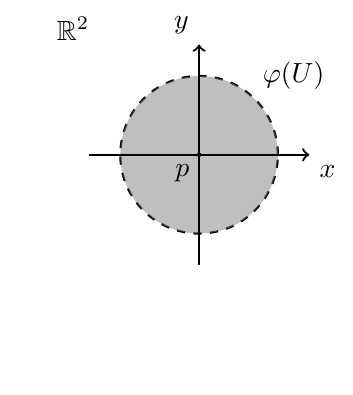
\begin{tikzpicture}[scale=0.4]
            % Draw the xy-plane grid
            
            % Draw the x and y axes
            
            % Draw a dashed circle in the XY-plane
            \draw[dashed, thick] (0,0) circle (2.5);
            \fill[color=gray, opacity=0.5] (0,0) circle (2.5);
            
            \draw[thick, ->] (-3.5,0) -- (3.5,0) node[anchor=north west] {$x$};
            \draw[thick, ->] (0,-3.5) -- (0,3.5) node[anchor=south east] {$y$};
            \node[] at (0,-5.8) {};

            \node[] at (-4,4) {$\mathbb{R}^2$};
            \node at (3,2.5) {$\varphi(U)$};
            % Mark the origin
            \fill[] (0,0) circle (2pt) node[anchor=north east] {$p$};
        \end{tikzpicture}
    \end{center}

    \caption{Sphere as a two manifold}
\end{figure}

\pagebreak
The tuple $(U,\varphi)$ in the above two examples is called a \emph{chart} on the manifold. The name comes from the cartographic chart and, similar to it, this chart allows us to map coordinates onto the neighborhood $U$. In a way of speaking, the chart and coordinates have made $U$ “navigable”. Note that, in the above figures, since $\varphi(U)$ are open sets, they are homeomorphic to the entire Euclidean space. Formally, we have the following definitions.

\begin{definition}{Chart}
    Let $\mathcal{M} \subseteq \mathbb{R}^n$. A chart on $\mathcal{M}$ is a pair $(U, \varphi)$ where $U$ is an open subset of $\mathcal{M}$ and $\varphi: U \to \mathbb{R}^n$ is a homeomorphism. $U$ is called a coordinate neighbourhood, and $\varphi$ is called a coordinate map.  A chart is said to be centered at $p \in \mathcal{M}$ if $\varphi(p) = 0$.
\end{definition}

\begin{definition}{Transition map}
    Let $\mathcal{M} \subseteq \mathbb{R}^n$. Let $(U, \varphi)$ and $(V, \psi)$ be two charts on $\mathcal{M}$, such that $U \cap V \neq \emptyset$. The transition map from $(U, \varphi)$ to $(V, \psi)$ is the map $\psi \circ \varphi^{-1}: \varphi(U \cap V) \to \psi(U \cap V)$. The two charts are said to be smoothly compatible if the transition map is smooth, or if the map $\psi \circ \varphi^{-1}$ is a diffeomorphism. 
\end{definition}

\begin{definition}{Atlas}
    An Atlas $\mathcal{A}$ for an $n$-manifold $\mathcal{M}$ is a collection of charts $(U_i, \varphi_i)$ on $\mathcal{M}$, such that each $U_i$ is homeomorphic to $\mathbb{R}^n$ and $\bigcup  U_i = \mathcal{M}$. The atlas is said to be smooth if all the transition maps between the charts are smooth, that is, the charts are smoothly compatible.
\end{definition}

The term \emph{Atlas} too comes from cartography, which is a collection of charts that map the entire world. The above definitions, assign a coordinate system on the entire manifold, which can be used to define smoothness on it.

\begin{definition}{Smooth structure}
    A smooth structure on a topological manifold $\mathcal{M}$ is a maximal smooth atlas $\mathcal{A}$ on $\mathcal{M}$. That is, $\mathcal{A}$ is a smooth atlas on $\mathcal{M}$ such that for any other smooth atlas $\mathcal{A'}$ on $\mathcal{M}$, $\mathcal{A} \subset \mathcal{A'}$.
\end{definition}

There can always be multiple Atlases on a manifold. The smooth structure is defined so that it is a unique Atlas that identifies the manifold. 
    
\subsection{Smooth manifolds}
\begin{definition}{Smooth manifold}
    A smooth manifold is a pair $(\mathcal{M}, \mathcal{A})$ where $\mathcal{M}$ is a topological manifold and $\mathcal{A}$ is a smooth structure on $\mathcal{M}$.
\end{definition}

Our pursuit of an analog to the FTC requires a little more structure in our manifold, that is of a boundary. For this, we need to define an analog to $\mathbb{R}^n$, which does have a boundary. This would be the Half-space $\mathbb{H}^n$ or $\mathbb{R}^n_+$. 

\begin{definition}{Closed $n$-dimientional half-space}
    The Closed $n$-dimientional Half-space is the set of all points in $\mathbb{R}^n$ such that the last coordinate is non-negative. That is, $\mathbb{H}^n = \{ (x_1, x_2, \ldots, x_n) \in \mathbb{R}^n | x_n \geq 0 \}$. 
    
    For $n = 1$, $\mathbb{H}^1 = [0, \infty)$. For $n = 2$, $\mathbb{H}^2 = \{ (x, y) \in \mathbb{R}^2 | y \geq 0 \}$, so the upper Half-Plane. And so on.    
\end{definition}

\begin{definition}{Manifold with boundary}
    A manifold with boundary is a topological space $\mathcal{M}$ such that every point $p \in \mathcal{M}$ has a neighborhood homeomorphic to an open subset of the closed half-space $\mathbb{H}^n$.
\end{definition}

\begin{definition}{Interior and boundary}
    Let $\mathcal{M}$ be a smooth manifold with a boundary. Let the Atlas on $\mathcal{M}$ be $\mathcal{A} = \{ (U_i, \varphi_i) \}$. 
    \begin{itemize}
        \item The interior of $\mathcal{M}$, denoted $\mathcal{M}^{\circ}$, is the set of all points $p \in \mathcal{M}$ such that there exists a chart $(U, \varphi) \in \mathcal{A}$ containing $p$ such that $\varphi(p) \in \mathbb{R}^n$ and $\varphi(U) \subset \mathbb{R}^n$.
        \item The boundary of $\mathcal{M}$, denoted $\partial \mathcal{M}$, is the set of all points $p \in \mathcal{M}$ such that for every chart $(U, \varphi) \in \mathcal{A}$ containing $p$, $\varphi(p) \in \mathbb{H}^n$ and $\varphi(p) \in \partial \mathbb{H}^n$, where $\partial \mathbb{H}^n = \{ (x_1, x_2, \ldots, x_n) \in \mathbb{R}^n \ | \ x_n = 0 \}$.
    \end{itemize}
\end{definition}

The boundary of the half-space is the set of all points where the last coordinate is zero. The boundary of a smooth manifold $\mathcal{M}$ with boundary, $\partial \mathcal{M}$, is thus the set of points in $\mathcal{M}$ that locally resemble points on the boundary of the closed upper half-space $\mathbb{H}^n$. These boundary points form an $(n-1)$-dimensional smooth manifold without boundary, embedded within the $n$-dimensional manifold $\mathcal{M}$.

\subsection{Tangent space}

The tangent space at a point on a manifold is a vector space that is isomorphic to the tangent surface at that point. The tangent to surfaces is intuitively understood as the direction of motion on the surface. Imagine a particle moving along a surface, with forces acting on it that constrain its motion onto the surface. If at a point the forces are removed, the direction in which the particle moves is the tangent to the surface at that point. In a motion on a circle, this is a line. If the motion is along a sphere, the direction depends on the path but always lies on a tangent plane. On a point on a sphere, there are two degrees of freedom for the direction of the path of motion, which makes the tangent surface a plane. To find tangent surfaces for a Euclidean surface, the ambient space plays a role and it is found by using the gradient of the function to find the normal and thus the tangent. Similar ideas are used to define the tangent space at a point on a manifold.

Consider a smooth manifold $\mathcal{M}$. Let $\gamma: \mathbb{R} \to \mathcal{M}$ be a parametrised path on $U$ such that WLOG, $\gamma(0) = p$. If the manifold is imagined to be a surface in $\mathbb{R}^n$, then just differentiating $\gamma$ in $\mathbb{R}^n$ would give the tangent to the surface at $p$. However because the manifold moves away from the ambient space, a different approach is needed. Though we cannot differentiate the curve, we can differentiate a function along it. Consider a function $f: \mathcal{M} \to \mathbb{R}$, such that $f \in C^{\infty}(\mathcal{M})$.

\[
\mathbb{R} \xrightarrow{\gamma}
\mathcal{M}
\xrightarrow{f \in C^{\infty}(\mathcal{M})} \mathbb{R}
\]

If we consider the composition $f \circ \gamma: \mathbb{R} \to \mathbb{R}$, then its derivative can be computed without problems. And evaluating it at $0$ evaluates it at $p$. This derivative measures the rate of change of $f$ along the curve $\gamma$ at $p$. But $(f\circ \gamma)'(0)$ is a number, and we want a vector. To recover a vector from this, this can be viewed as an action on the function $f$, which is the directional derivative along the curve $\gamma$. Consider a new notation of the above.
\[
    X_{\gamma, p}(f) := (f \circ \gamma)'(0).
\]
These vectors are not points sticking out of $p$ in a tangent surface but are rather derivative functions. But they do carry a sense of the tangential direction with them. $X_{\gamma, p}$ is a map that measures the rate of change of a function along the direction shown in the figure above.

\begin{figure}[h]
    \centering
    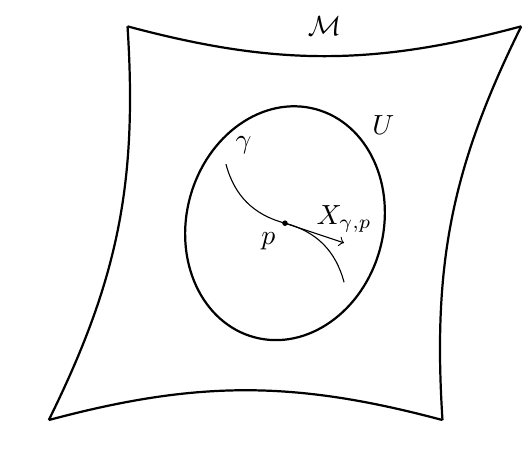
\begin{tikzpicture}[scale=0.5]
        \draw[thick, bend left=15] (-6,-5) to (4,-5) ;
        \draw[thick, bend right=15] (-4,5) to (6,5);
        \draw[thick, bend right=15] (-6,-5) to (-4,5);
        \draw[thick, bend right=15] (6,5) to (4,-5);     
    
        
        \fill (0,0) circle (2pt) node[below left] at (0,0) {$p$};
        \node[] at (1,5) {$\mathcal{M}$};
        \node[] at (2.5,2.5) {$U$};
        % \draw[] (0,0) circle (3); this should be an oval rotated by 15 deg to the right
        % \draw[thick] (0,0) ellipse (2.5 and 3);
        \draw[thick, rotate around={75:(0,0)}] (0,0) ellipse (3 and 2.5);

        \draw[bend right] (-1.5, 1.5) node[above right] {$\gamma$} to (0,0);
        \draw[bend right] (1.5, -1.5) to (0,0);
    
        \draw[->] (0,0) -- (1.5, -0.5) node[above=0.3pt] {$X_{\gamma, p}$};
    \end{tikzpicture}
    \caption{The ``direction'' of $X_{\gamma, p}$}
\end{figure}
\pagebreak
\noindent Note that because the derivative is linear, $X_{\gamma, p}$ is a linear map. So,
\begin{align*}
    X_{\gamma, p}(f + g) &= X_{\gamma, p}(f) + X_{\gamma, p}(g) \\
    X_{\gamma, p}(af) &= aX_{\gamma, p}(f).
\end{align*}
Now the tangent space at $p$  is defined as the set $T_p\mathcal{M} = \{X_{\gamma,p} | \  \gamma \text{ is a smooth path on \(\mathcal{M}\) and } \gamma (0) = p\}$. It is formed by taking all paths through $p$ and their corresponding directional derivative operators. Though lengths of these vectors are not defined yet, it is intuitive to see that if we take $\gamma'(t) = \gamma(2t)$, a path moving twice as fast, then $X_{\gamma, p}f = 2X_{\gamma', p}f$. So in each direction, the whole line is spanned by these vectors, and collectively they span the whole tangent surface. Even though the tangent space is not a surface tangent to the manifold, we see that it ``looks like" it. The tangent space is a vector space itself, where addition and scalar multiplication are defined as follows.
\begin{align*}
    (X_{\gamma, p} + X_{\gamma', p})(f) &= X_{\gamma, p}(f) + X_{\gamma', p}(f) \\
    (aX_{\gamma, p})(f) &= aX_{\gamma, p}(f).
\end{align*}
\subsubsection{Basis of the tangent Space}
At each point $p \in \mathcal{M}$, the tangent space $T_p\mathcal{M}$ is a vector space. A basis for this vector space is induced by the chart on the manifold. Let $(U, \varphi)$ be a chart on $\mathcal{M}$ from its smooth structure, centered at point $p$. $\varphi$ takes points in $U$ to $\mathbb{R}^n$ and WLOG, $\varphi(p) = \mathcal{O}$. Consider the axes of $\mathbb{R}^n$, and lift them back onto the manifold using $\varphi^{-1}$.
\begin{figure}[h]
    \centering
    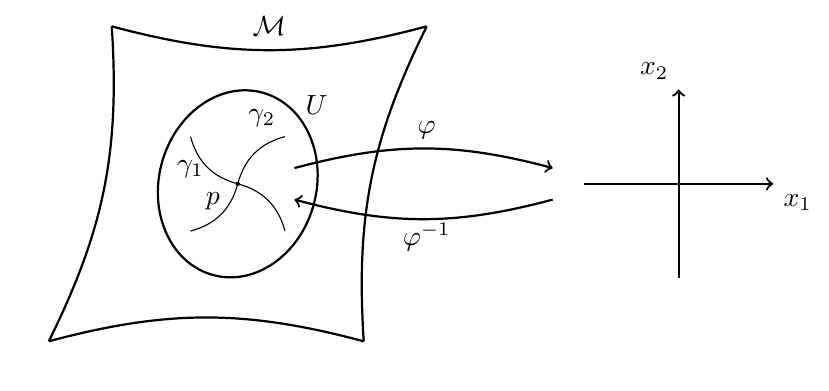
\begin{tikzpicture}[scale=0.4]
        \draw[thick, bend left=15] (-6,-5) to (4,-5) ;
        \draw[thick, bend right=15] (-4,5) to (6,5);
        \draw[thick, bend right=15] (-6,-5) to (-4,5);
        \draw[thick, bend right=15] (6,5) to (4,-5);     
    
        
        \fill (0,0) circle (2pt) node[below left=-0.3pt and 3pt] at (0,0) {$p$};
        \node[] at (1,5) {$\mathcal{M}$};
        \node[] at (2.5,2.5) {$U$};
        \draw[thick, rotate around={75:(0,0)}] (0,0) ellipse (3 and 2.5);

        \draw[bend right] (-1.5, 1.5) node[below=5pt] {$\gamma_1$} to (0,0);
        \draw[bend right] (1.5, -1.5) to (0,0);
        \draw[bend right] (-1.5, -1.5) to (0,0);
        \draw[bend right] (1.5, 1.5) node[above left] {$\gamma_2$} to (0,0);
        \draw[thick, bend right=15, <-] (1.8,-0.5) to (10, -0.5) ;
        \draw[thick, bend right=15, <-] (10, 0.5) to (1.8,0.5) ;
        \node[] at (6,1.7) {$\varphi$};
        \node[] at (6,-1.7) {$\varphi^{-1}$};

        
        \draw[thick, ->] (11,0) -- (17,0) node[anchor=north west] {$x_1$} node[above, midway] {};
        \draw[thick, ->] (14,-3) -- (14,3) node[anchor=south east] {$x_2$};
    \end{tikzpicture}
    \caption{Paths corresponding to the axes}
\end{figure}

\noindent $\gamma_i$, the path on $U$ of the lifted $x_i$ chart axis, can be defined as follows.
\begin{align*}
    \gamma_i(t) : \mathbb{R} &\to U\\
     t \  &\to \varphi^{-1}(0, \ldots, \underbrace{t}_{i^{th} \ entry}, \ldots, 0)
     = \ \varphi^{-1}(\delta^1_{i}t, \ldots, \delta^i_{i}t, \ldots, \delta^n_{i}t)\\
\end{align*}
The projection of a point on this path onto a coordinate axes is a useful action to look at, for later use. 
\begin{align*}
    (x^a\circ \gamma_i)(t) &= \delta_i^a t\\
    \implies (x^a\circ \gamma_i)' &= \delta_i^a \ .
\end{align*}
Now if tangent vectors are constructed from these paths, $X_{\gamma_i, p}$, then these form a basis for the tangent space at $p$. Let $f \in C^{\infty}(\mathcal{M})$, be a smooth function. Consider the action of $X_{\gamma_i, p}$ on $f$:
\begin{align*}
    X_{\gamma_i, p}(f) &= (f \circ \gamma_i)'(0)\\
    &= (f\circ \varphi \circ \varphi^{-1} \circ \gamma_i)'(0). 
\end{align*}
$f\circ \varphi^{-1}$ is a function from $\mathbb{R}^n \to \mathbb{R}$ and $\varphi \circ \gamma_i$ is a function from $\mathbb{R}\to \mathbb{R}^n$. So the above derivative can be treated as a derivative of two multivariate functions, and the chain rule can be used. So,
\begin{align*}
    X_{\gamma_i, p}(f) &= (f\circ \varphi^{-1} \circ \varphi \circ \gamma_i)'(0)\\
    &= \sum \frac{\partial}{\partial x^a} \left(f\circ \varphi^{-1}\right)((\varphi\circ\gamma_i)(0))\cdot (\varphi\circ\gamma_i)'(0)\\
    &= \sum \frac{\partial}{\partial x^a} \left(f\circ \varphi^{-1}\right)(\varphi(p))\cdot (\varphi^a\circ\gamma_i)'(0)\\
    &= \sum \frac{\partial}{\partial x^a} \left(f\circ \varphi^{-1}\right)(\varphi(p))\cdot (\delta_i^a)\\
    &= \frac{\partial}{\partial x^i} \left(f\circ \varphi^{-1}\right)(\varphi(p)) .\\
\end{align*}
For a shorter notation, we denote
$X_{\gamma_i, p}$ as $\dfrac{\partial}{\partial x^i}\bigg|_p$. It can be shown that $\left\{\dfrac{\partial}{\partial x^1}\bigg|_p, \dfrac{\partial}{\partial x^2}\bigg|_p, \ldots, \dfrac{\partial}{\partial x^n}\bigg|_p\right\}$ is a basis for the tangent space at  $p$. The reader can find this proof in Hubbards' book \cite{hubbard2009vector}.
This is called the coordinate basis or the chart-induced basis. The tangent space at $p$ is then spanned by these vectors. $T_p\mathcal{M}$ is then a vector space of dimension $n$.
\subsection{Orientation, orientability}

Tu's book \cite{tu2010introduction} was consulted for this section. Recall that in the normal integration of a function($f: \mathbb{R} \to \mathbb{R}$) over an interval, we have a notion of orientation built into the integral. The integral of f over $[a, b]$, and is negative of the integral of $f$ over $[b, a]$. This even exists in the iterated Riemann integration that is defined on functions from $\mathbb{R}^n$ to $\mathbb{R}$. Switching the bounds of the integral switches its sign. So a notion of orientation is built into the integral, and the integral measures the ``oriented" volume under the function.

Let us look at a few base examples. Consider $\mathbb{R}^1$, a line. There are two orientations here, corresponding to the left and right directions. Now consider $\mathbb{R}^2$, a plane. This also has two orientations, corresponding to the clockwise and anticlockwise directions. Consider $\mathbb{R}^3$, a 3-dimensional space. There are two orientations here, corresponding to the right-hand and left-hand rules. 

These rules are just a choice on how the standard basis of $\mathbb{R}^n$ is ordered. For $\mathbb{R}^1$ an orientation could be given by either $e_1$ or $-e_1$. For $\mathbb{R}^2$ the counterclockwise orientation is $(e_1, e_2)$, while the clockwise orientation is $(e_2, e_1)$. For $\mathbb{R}^3$, the right-handed orientation is $(e_1, e_2, e_3)$, and the left-handed orientation is $(e_2, e_1, e_3)$. To visualize this, imagine placing the middle finger, index finger, and thumb along the axes in $\mathbb{R}^3$, corresponding to the above-specified order. That is, for $(e_1, e_2, e_3)$, middle finger is placed along $e_1$, index along $e_2$ and thumb along $e_3$. If we use the left hand, we see that it works fine for the first ordering but in the second ordering forces the thumb opposite to the $e_3$ direction. 

\begin{figure}
    \centering
    \includegraphics[width=0.5\linewidth]{images/r3ori.png}
    \caption{Orientations of $\mathbb{R}^3$}
\end{figure}
\begin{definition}{Orientation}
    Consider a general vector space $V$. An orientation on $V$ is defined by an equivalence relation on the set of ordered bases of $V$. Let $B_1 = (v_1, v_2, \ldots, v_n)$ and $B_2 = (w_1, w_2, \ldots, w_n)$ be two ordered bases of $V$. Recall that the change of basis matrix from $B_1$ to $B_2$ is the matrix $A$ such that $[w_1, w_2, \ldots, w_n] = [v_1, v_2, \ldots, v_n]A$. 

    $B_1 \sim B_2$ if the change of basis matrix from $B_1$ to $B_2$ has positive determinant. Under this equivalence relation, an orientation on $V$ is defined as an equivalence class of ordered bases of $V$. 
\end{definition}
\subsubsection{Orienting a manifold}

To extend the notion of orientation to manifolds, the tangent space at each point is given orientation. This has to be done in a way that it is ``consistent" and there is no abrupt change in orientation as we move along the manifold.

\begin{definition}{Frame}
    Let $\mathcal{M}$ be a smooth manifold, and $U \subset \mathcal{M}$ be an open subset. A frame on $U$ is an n-tuple of (possibly discontinuous) vector fields $(X_1, X_2, \ldots, X_n)$ on $U$ such that at each point $p \in U$, the vectors $(X_1(p), X_2(p), \ldots, X_n(p))$ form a basis for the tangent space $T_p\mathcal{M}$. A \textit{global frame} is a frame on the entire manifold $\mathcal{M}$, whereas a \textit{local frame} is a frame on an open subset $U \subset \mathcal{M}$.
\end{definition}

\noindent The following equivalence relation on frames is defined to extend the notion of orientation to manifolds. $\forall p \in U$,
$$
(X_1, X_2, \ldots, X_n) \sim (Y_1, Y_2, \ldots, Y_n) \iff (X_1(p), X_2(p), \ldots, X_n(p)) \sim (Y_1(p), Y_2(p), \ldots, Y_n(p)) .
$$

\noindent That is, at each point $p \in U$, the change of basis matrix from $(X_1(p), X_2(p), \ldots, X_n(p))$ to \\$(Y_1(p), Y_2(p), \ldots, Y_n(p))$ has positive determinant.

\begin{definition}{Point-wise orientation}
    A point-wise orientation on a manifold $\mathcal{M}$, assigns to each point $p \in \mathcal{M}$ an orientation $\mu_p$ on the tangent space $T_p\mathcal{M}$. So, the pointwise orientation is a (possibly discontinuous) equivalence class of frames on $\mathcal{M}$.
\end{definition}
\noindent The point-wise orientation $\mu$ is said to be continuous at a point $p \in \mathcal{M}$ if there exists a neighborhood $U$ of $p$ on which the orientation is represented by a continuous frame. That means there exist continuous vector fields $X_1, X_2, \ldots, X_n$ on $U$ such that $\forall q \in U$, the equivalence class $[(X_1(q), X_2(q), \ldots, X_n(q))]$ represent the orientation at $q$. 

\noindent If the point-wise orientation is continuous at every point $p \in \mathcal{M}$, the point-wise orientation is said to be continuous on $\mathcal{M}$. If such a point-wise orientation exists, it is said to be an \textit{orientation} on $\mathcal{M}$, and the manifold is said to be \textit{orientable}.



\begin{definition}{Orientation on a manifold with boundary}
    Given a manifold with boundary $\mathcal{M}$, its orientation is a smoothly compatible choice of orientations at each of its tangent spaces $T_p\mathcal{M}$. 
    If the choice of orientation for a manifold satisfies smooth compatibility, the coordinate charts are said to be \emph{orientation-preserving}. Every orientation induces an orientation on its boundary, which is either directed outward or inward on the boundary. These are referred to as the outward and inward normals.
\end{definition}
The following results are stated without proof, for later use.

\begin{theorem}{}
    \begin{itemize}
    \item A connected, orientable manifold with boundary allows for only two possible orientations.
    \item An orientable smooth manifold with boundary $\mathcal{M}$ has a smooth outward-pointing vector field on $\partial \mathcal{M}$ 
\end{itemize}
\end{theorem}
\begin{definition}{Dual space}
    Let $V$ be a vector space. The dual space of $V$, denoted $V^*$, is the set of all linear functions on $V$. That is, $$V^* = \{ f: V \to \mathbb{R} \ | \ f \text{ is linear}. \}$$.
\end{definition} 

\section{Exterior algebra}
To introduce differential forms, the idea of multilinear functions is introduced and an algebra on them is defined. This section is based on the books of Hubbards \cite{hubbard2009vector} and Tu \cite{tu2010introduction}.
\subsection{Tensors}
\begin{definition}{Tensors}
    Let $V$ be a vector space over reals. $V^k = V\times \dots \times V$, the  $k-$fold cartesian product of $V$ with itself. A real-valued function $T: V^k \to \mathbb{R}$ is said to be  $k-$linear if it is linear in each of its  $k-$arguments. That is, in each slot, 
    \[
        T(\dots, a v + w, \dots) = a T(\dots, v, \dots) + T(\dots, w, \dots),
    \]
    where $v, w \in V$ and $a \in \mathbb{R}$. A $k-$linear function is also called a $k-$tensor. k is referred to as the \textit{rank} of the $k-$tensor. The set of p-vectors on V is denoted by $\mathcal{T}^p (V)$
\end{definition}

The aim of introducing tensors is to generalize a few  $k-$linear vector functions that are already seen. For example, the inner product, which is a 2-tensor; the determinant, which is a  $k-$tensor. Now, an operation on tensors called the tensor product is introduced as a way to combine two tensors.

\begin{definition}{Tensor product}
    Let T $\in \mathcal{T}^k (V)$ and S $\in \mathcal{T}^l (V)$. The tensor product of T and S, denoted $T \otimes S$, is a $(k+l)$-tensor defined as follows:
    \[
        (T \otimes S)(v_1, v_2, \ldots, v_{k+l}) = T(v_1, v_2, \ldots, v_k) S(v_{k+1}, v_{k+2}, \ldots, v_{k+l}).
    \]
    It can be shown that the tensor product is associative and distributive. That is, If $T, S, R$ are some tensors, then
    \begin{align*}
        (T \otimes S) \otimes R &= T \otimes (S \otimes R) \\
        T \otimes (S + R) &= T \otimes S + T \otimes R.
    \end{align*}
\end{definition}
\subsubsection{The Alt tensor}
Tensors can be classified into two types based on their properties under permutations of their arguments.

\begin{definition}{Symmetric and alternating tensors}
    Let T $\in \mathcal{T}^k (V)$. $S_k$ is the symmetric group on k elements, containing the permutations.

    T is said to be \emph{symmetric,} if for any $\sigma \in S_k$, $$T(v_{\sigma(1)}, v_{\sigma(2)}, \ldots, v_{\sigma(k)}) = T(v_1, v_2, \ldots, v_k).$$
    $\Lambda^k(V^*)$ is denoted as the space of alternating  $k-$tensors on V. The asterisk comes from the deal space and indicates multilinearity.

    T is said to be \emph{alternating,} if for any $\sigma \in S_k$, $$T(v_{\sigma(1)}, v_{\sigma(2)}, \ldots, v_{\sigma(k)}) = \text{sgn}(\sigma) T(v_1, v_2, \ldots, v_k).$$
\end{definition}

Now, the \textit{Alt} operation on a tensor is introduced, which allows us to convert a tensor into an alternating tensor. 

\begin{definition}{Alt(T)}
    Let T $\in \mathcal{T}^k (V)$. The Alt(T) is a  $k-$tensor on $V$ defined as follows.
    \begin{align*}
        (\text{Alt}(T))(v_1, v_2, \ldots, v_k) &= \frac{1}{k!} \sum_{\sigma \in S_k} \text{sgn}(\sigma) \ T(v_{\sigma(1)}, v_{\sigma(2)}, \ldots, v_{\sigma(k)})\\
        \text{Alt}(T) &= \frac{1}{k!} \sum_{\sigma \in S_k} \text{sgn}(\sigma) \ \sigma T.
    \end{align*}
    Here, $S_k$ is the symmetric group on k elements. $\sigma T$ permutes the arguments of Alt T through the permutation $\sigma$ and passes them to T. Alt is called the alternation operator, as it converts any tensor $T$ into an alternating tensor. If T itself is an alternating tensor, then Alt(T) = T.
\end{definition}
\begin{proposition}
    Alt(T) is an alternating tensor.    
\end{proposition}
\begin{proof}
    Consider Alt(T) constructed as above and let $\sigma \in S_k$. To show that $\sigma \text{Alt}(T) = sgn(\sigma) \text{Alt}(T)$.
    \begin{align*}
        \sigma \text{Alt}(T)(v_1, v_2, \ldots, v_k) &= Alt(T)(v_{\sigma(1)}, v_{\sigma(2)}, \ldots, v_{\sigma(k)}) \\
        &= \frac{1}{k!} \sum_{\tau \in S_k} \text{sgn}(\tau) \ T(v_{\tau(\sigma(1))}, v_{\tau(\sigma(2))}, \ldots, v_{\tau(\sigma(k))}). \\
    \end{align*}
    Now, since sgn$(\sigma)^2$ is equal to $1$, we can multiply the sum by sgn$(\sigma)^2$. Also, sgn$(\sigma \tau)$ is equal to $\text{sgn}(\sigma) \text{sgn}(\tau)$, 
    \begin{align*}
        \sigma \text{Alt}(T)(v_1, v_2, \ldots, v_k) &= \frac{1}{k!} \sum_{\tau \in S_k} \text{sgn}(\tau) \text{sgn}(\sigma)\cdot \text{sgn}(\sigma) \ T(v_{\tau(\sigma(1))}, v_{\tau(\sigma(2))}, \ldots, v_{\tau(\sigma(k))}) \\
        &= \text{sgn}(\sigma) \frac{1}{k!} \sum_{\tau \in S_k} \text{sgn}(\tau \circ \sigma) \ T(v_{\tau \circ \sigma(1)}, v_{\tau \circ \sigma(2)}, \ldots, v_{\tau \circ \sigma(k)}) \\
        &= \text{sgn}(\sigma) \frac{1}{k!} \sum_{\pi \in S_k} \text{sgn}(\pi) \ T(v_{\pi(1)}, v_{\pi(2)}, \ldots, v_{\pi(k)}) \\
        &= \text{sgn}(\sigma) \text{Alt}(T)(v_1, v_2, \ldots, v_k).
    \end{align*}
    Hence, $\sigma \text{Alt}(T)$ is equal to $\text{sgn}(\sigma) \text{Alt}(T)$, and Alt(T) is an alternating tensor.
\end{proof}


\subsection{Wedge product}
With the preliminaries in place, the wedge product can now be introduced. The wedge product is also used to combine two tensors, but the result has more properties, that of being an alternating tensor.

\begin{definition}{Wedge product}
    Consider T$\in \mathcal{T}^k (V)$ and S$\in \mathcal{T}^l (V)$. The wedge product of T and S, denoted $T \wedge S$, is a $(k+l)$-tensor defined as 
    \[
        T \wedge S = Alt(T \otimes S).
    \]    
\end{definition}
A few properties of the wedge product are listed without proof.
\begin{itemize}
    \item If Alt$(T) = 0$, then $T \wedge S = 0 = S \wedge T$.
    \item The wedge product is associative. Additionally, 
    $$(T \wedge S) \wedge R = T \wedge (S \wedge R) = \text{Alt}(T\otimes S\otimes R).$$
    \item The wedge product is anti-commutative. That is,
    $$T \wedge S = (-1)^{kl} S \wedge T.$$
\end{itemize}
 

\section{Differential forms}

We now revert to the setting of the manifold and apply the tools developed in exterior algebra there. This section first introduces differential forms on $\mathbb{R}^n$ and then extends the idea to manifolds. The contents of this section were inspired by Shifrin's \cite{shifrin2004multivariable} and Hubbards' \cite{hubbard2009vector} books.

Differential forms are mathematical objects that help us give meaning to the integrand and the integral. They are a generalization of the  $k-$volume element present in the integrand of the iterated Riemann integration. 
\subsection{Differential forms on $\mathbb{R}^n$}
\subsubsection{Dual space of $\mathbb{R}^n$}
The dual space of $\mathbb{R}^n$, $(\mathbb{R}^n)^*$, is the set of all linear functions on $\mathbb{R}^n$. That is, $(\mathbb{R}^n)^*$ is the set $\{ f: \mathbb{R}^n \to \mathbb{R} \ | \ f \text{ is linear} \}$. For example, the dot product is a linear function on $\mathbb{R}^n$. So if you take any vector $a \in \mathbb{R}^n$, the function $f_a: \mathbb{R}^n \to \mathbb{R}$ is a linear function on $\mathbb{R}^n$ defined by
$$f_a(x) = a \cdot x.$$ 
Hence $f_a \in (\mathbb{R}^n)^*$. The matrix corresponding to this linear function is the row vector $a$.

\noindent The dual space itself is a vector space, with the operations of addition and scalar multiplication defined pointwise. That is, if $f, g \in (\mathbb{R}^n)^*$ and $a \in \mathbb{R}$, then $(f + g)(x) $ is equal to $ f(x) + g(x)$, and $(af)(x)$ is equal to $a f(x)$ for all $x \in \mathbb{R}^n$. The dual space is isomorphic to $\mathbb{R}^n$ itself, as each linear function  $f \in (\mathbb{R}^n)^*$ can be identified with the row vector $[f(e_1), f(e_2), \ldots, f(e_n)]$. So $\dim (\mathbb{R}^{n*})$ is $n$.

\subsubsection{The standard basis of the dual space}
From the isomorphism, it can be concluded that each basis of $\mathbb{R}^n$ has a corresponding dual basis of $(\mathbb{R}^{n*})$. So consider the standard basis of $\mathbb{R}^n$, $e_1,\  e_2, \ \cdots, \ e_n$. The corresponding dual basis of $(\mathbb{R}^{n*})$ is the set of linear functions $\epsilon_1, \ \epsilon_2, \ \cdots, \ \epsilon_n$ such that $\epsilon_i(x) $ is equal to $ \langle e_i, x \rangle$ for all $x \in \mathbb{R}^n$. 

\noindent Let $(dx^1, dx^2, \ldots, dx^n)$ be a notation for the dual basis. The dual basis is also called the \textit{co-ordinate basis} of $(\mathbb{R}^{n*})$. So,
$$dx^i(x) = \langle e_i, x \rangle = x^i .$$ 

The dual space of $\mathbb{R}^n$ is simply the space of 1-tensors on $\mathbb{R}^n$. This space is also the same as $\Lambda^1(\mathbb{R}^{n*})$ since the alternating 1-tensors on $\mathbb{R}^n$ are the same as the 1-tensors.
A similar structure for $\Lambda^k(\mathbb{R}^{n*})$ is needed. Recall that the determinant is an alternating and multilinear function that we have already seen. It is thus only natural that it shows up here. 

As an example, let $k=2, n=3$. So we are looking at 2-tensors on $\mathbb{R}^3$. These are alternating and bilinear functions, that take in two vectors and give out a scalar. The determinant function $D(v_1, v_2) = \det[v_1, v_2, a]$, where $a$ is any vector in $\mathbb{R}^3$, is a 2-tensor on $\mathbb{R}^3$. From our knowledge of determinants, this function is known to be real-valued, alternating, and bilinear. The vector $a$ can be any vector, so let us look at what happens when $a = e_1$. Let $D_1$ be the 2-tensor,
\begin{align*}
    D_1(v_1, v_2) = \begin{vmatrix}
        v_{11} & v_{21} & 1\\
        v_{12} & v_{22} & 0\\
        v_{13} & v_{23} & 0
    \end{vmatrix} = \begin{vmatrix}
        v_{12} & v_{22}\\
        v_{13} & v_{23}
    \end{vmatrix}.\\
\end{align*}
So if the following matrix of the vectors $v_1$ and $v_2$ is considered, 
\[
    \begin{bmatrix}
        v_{11} & v_{21}\\
        v_{12} & v_{22}\\
        v_{13} & v_{23}
    \end{bmatrix}
\]
$D_1$ takes the second and third rows of this matrix and computes the determinant of the resulting $2\times2$ matrix. From this, a new notation for $D_1$ is introduced: $dx_{2,3}$. So $dx_{2,3}(v_1, v_2) = \begin{vmatrix}
    v_{12} & v_{22}\\
    v_{13} & v_{23}
\end{vmatrix}$. This is a 2-tensor on $\mathbb{R}^3$. Note that our $dx_1$ notation from earlier, still follows this form of choosing rows for the determinant, because the dot product with $e_i$ is the same as choosing the $i^{th}$ entry of the vector for the 1x1 determinant. 
Now consider all such functions that choose two rows of the matrix and compute the determinant.
\[
\begin{array}{ccc}
    dx_{1,1} & dx_{1,2} & dx_{1,3}\\
    dx_{2,1} & dx_{2,2} & dx_{2,3}\\
    dx_{3,1} & dx_{3,2} & dx_{3,3}
\end{array}
\]
If the rows are the same, then the determinant is zero, so $dx_{1,1}, dx_{2,2}, dx_{3,3}$ are always zero. Also, t $dx_{i,j} = -dx_{j,i}$. It can be shown that $dx_{1,2}, dx_{1,3}, dx_{2,3}$ form a basis of $\Lambda^2(\mathbb{R}^{3*})$. 

This notation is generalised to $\Lambda^k(\mathbb{R}^{n*})$. Let $I = (i_1, i_2, \ldots, i_k)$ be an increasing multi-index, that is $1 \leq i_1 < i_2 < \ldots < i_k \leq n$. Then $dx_I$ is a $k-$tensor on $\mathbb{R}^n$ defined as 
\[
    dx_I(v_1, v_2, \ldots, v_k) = \begin{vmatrix}
        v_{1i_1} & v_{2i_1} & \ldots & v_{ki_1}\\
        v_{1i_2} & v_{2i_2} & \ldots & v_{ki_2}\\
        \vdots & \vdots & \ddots & \vdots\\
        v_{1i_k} & v_{2i_k} & \ldots & v_{ki_k}
    \end{vmatrix}.
\]

\begin{proposition}{$dx_{i_1, i_2, \ldots, i_k} = dx_{i_1} \wedge dx_{i_2} \wedge \ldots \wedge dx_{i_k}$}
\end{proposition}
\begin{proof}
    Let $A = [a_{mn}] = [v_{n i_m}]$.
    \begin{align*}
        LHS = dx_{i_1, i_2, \ldots, i_k}(v_1, v_2, \ldots, v_k) &= \det(A)\\
        &= \sum_{\sigma \in S_k} \text{sgn}(\sigma) a_{1\sigma(1)} a_{2\sigma(2)} \ldots a_{k\sigma(k)}\\
        &= \sum_{\sigma \in S_k} \text{sgn}(\sigma) v_{1i_{\sigma(1)}} v_{2i_{\sigma(2)}} \ldots v_{ki_{\sigma(k)}}\\
        &= \sum_{\sigma \in S_k} \text{sgn}(\sigma) dx_{i_{\sigma(1)}}(v_1) dx_{i_{\sigma(2)}}(v_2) \ldots dx_{i_{\sigma(k)}}(v_k).\\
    \end{align*}
    Now,
    \begin{align*}
        RHS = dx_{i_1} \wedge \ldots \wedge dx_{i_k}(v_1, v_2, \ldots, v_k) &= Alt(dx_{i_1} \otimes dx_{i_2} \otimes \ldots \otimes dx_{i_k})(v_1, v_2, \ldots, v_k)\\
        &= \sum_{\sigma \in S_k} \text{sgn}(\sigma) dx_1 \otimes dx_2 \otimes \ldots \otimes dx_k(v_{\sigma(1)}, v_{\sigma(2)}, \ldots, v_{\sigma(k)})\\
        &= \sum_{\sigma \in S_k} \text{sgn}(\sigma) dx_1(v_{\sigma(1)}) dx_2(v_{\sigma(2)}) \ldots dx_k(v_{\sigma(k)})\\
        &= \sum_{\sigma \in S_k} \text{sgn}(\sigma) dx_{\sigma^{-1}(1)}(v_1) dx_{\sigma^{-1}(2)}(v_2) \ldots dx_{\sigma^{-1}(k)}(v_k)\\
        &= \sum_{\pi \in S_k} \text{sgn}(\pi) dx_{i_{\pi(1)}}(v_1) dx_{i_{\pi(2)}}(v_2) \ldots dx_{i_{\pi(k)}}(v_k).\\
    \end{align*}
    We observe that the left and right sides are equal, and so $dx_{i_1, i_2, \ldots, i_k} = dx_{i_1} \wedge dx_{i_2} \wedge \ldots \wedge dx_{i_k}$.
\end{proof}

\noindent It can be shown that the set $\{dx_{i_1, i_2, \ldots, i_k} \ | \ 1 \leq i_1 < i_2 < \ldots < i_k \leq n\}$ forms a basis for $\Lambda^k(\mathbb{R}^{n*})$. But for the scope of this paper, this is stated without proof. From this, it can also be concluded that $\dim \Lambda^k(\mathbb{R}^{n*}) $ is equal to $ \binom{n}{k}$. These  $k-$tensors on $\mathbb{R}^n$ are called differential  $k-$forms on $\mathbb{R}^n$. This notion can now be extended to manifolds.

\subsubsection{Geometric interpretation}
The idea of the determinant as an \emph{oriented}  $k-$volume of the  $k-$parallelotope spanned by vectors $v_1, v_2, \ldots, v_k$ in $\mathbb{R}^k$, can be used to give a geometric meaning to differential  $k-$forms. To make visualization easy, consider $\mathbb{R}^3$ and the “standard” 0, 1, 2, and 3-forms on it($dx_I$ defined above).
\begin{itemize}
    \item $dx_i$ is a 1-form on $\mathbb{R}^3$. It takes a vector $v \in \mathbb{R}^3$ and returns the $i^{th}$ component of the vector, which is the projection of $v$ onto the $i^{th}$ axis. This length is a 1-volume.
    \item $dx_{i,j}$ is a 2-form on $\mathbb{R}^3$. It takes two vectors $v^1, v^2 \in \mathbb{R}^3$ and returns the determinant of the $2\times2$ matrix
    \(
        \begin{vmatrix}        
            v_{1i} & v_{2i}\\
            v_{1j} & v_{2j}
        \end{vmatrix}
    \). Considering only the $i^{th}$ and $j^{th}$ components of the vectors is nothing but taking the projection of the vectors onto the $x^i, x^j$ plane. This is just the area of the parallelogram on the $x^i, x^j$ plane spanned by the projections of $v_1, v_2$ onto the $x^i, x^j$ plane. Let $v^{i,j}$ denote the projection of $v$ onto the $x^i, x^j$ plane. Then we get the following figure. $dx_{1,2}(v_1, v_2)$ returns the gray area in the figure. Note that the area is just 2-volume.
\begin{center}
    \tdplotsetmaincoords{78}{140}
    \tdplotsetrotatedcoords{3}{0}{5} 
    \begin{tikzpicture}[tdplot_main_coords,line cap=round,>=stealth]
        \begin{scope}[tdplot_rotated_coords]
            % Define the coordinates for the vectors
            \coordinate (O) at (0,0,0);
            \coordinate (V1) at (2,1,1.5);
            \coordinate (V2) at (1,2.3,1.5);
            \coordinate (V1plusV2) at (3,3.3,3);
            \coordinate (V1proj) at (2,1,0);
            \coordinate (V2proj) at (1,2.3,0);
            \coordinate (V1plusV2proj) at (3.3,3.6,0);
            % Draw the axes
            \draw[thick] (0,0,0) -- (3,0,0)  node[pos=1.05]{$x^1$};
            \draw[dashed] (0,0,0) -- (-1,0,0) node[pos=1.05]{}; 
            \draw[thick] (0,0,0) -- (0,3,0) node[pos=1.05]{$x^2$};
            \draw[dashed] (0,0,0) -- (0,-1,0) node[pos=1.05]{}; 
            \draw[thick] (0,0, 0) -- (0,0,3) node[pos=1.05]{$x^3$};
            \draw[dashed] (0,0,-1) -- (0,0,0) node[pos=1.05]{};

            % Draw the vectors
            \draw[thick,->=0.5] (O) -- (V1) node[above] {$\mathbf{v}_1$};
            \draw[thick,->=0.5] (O) -- (V2) node[below right] {$\mathbf{v}_2$};
            \draw[dashed] (V1) -- (V1plusV2);
            \draw[dashed] (V2) -- (V1plusV2);
            \draw[thick,->=0.5] (O) -- (V1proj) node[below left] {$\mathbf{v}_1^{1,2}$};
            \draw[thick,->=0.5] (O) -- (V2proj) node[below right] {$\mathbf{v}_2^{1,2}$};
            \draw[thin] (V1proj) -- (V1plusV2proj);
            \draw[thin] (V2proj) -- (V1plusV2proj);

            % \draw[dashed] (V1) -- (V1proj);
            % \draw[dashed] (V2) -- (V2proj);
            % \draw[thin] (V1plusV2) -- (V1plusV2proj);

            % Draw the parallelogram
            \fill[red,opacity=0.2] (O) -- (V1) -- (V1plusV2) -- (V2) -- cycle;
            \fill[gray,opacity=0.3] (O) -- (V1proj) -- (V1plusV2proj) -- (V2proj) -- cycle;
        \end{scope}
    \end{tikzpicture}
\end{center}
    Similarly,  $dx_{2,3}(v_1, v_2)$ would take the projection onto the $x^2, x^3$ plane and return the area of the parallelogram. 
    \item $dx_{1,2,3}$ is a 3-form on $\mathbb{R}^3$. It takes three vectors $v_1, v_2, v_3 \in \mathbb{R}^3$ and returns the determinant of the $3\times3$ matrix
    \(
        \begin{vmatrix}        
            v_{11} & v_{21} & v_{31}\\
            v_{12} & v_{22} & v_{32}\\
            v_{13} & v_{23} & v_{33}
        \end{vmatrix}
    \). This is the oriented volume of the parallelepiped spanned by the vectors $v_1, v_2, v_3$. Another way of saying this would be the volume of the parallelepiped spanned by the projections of $v_1, v_2, v_3$ onto the $x^1, x^2, x^3$ space (which are just $v_1, v_2, v_3$ respectively).
\end{itemize}
In general, the standard  $k-$form on $\mathbb{R}^n$, $dx_{i_1, i_2, \ldots, i_k}$, takes $k$ vectors $v_1, v_2, \cdots, v_k \in \mathbb{R}^n$ and returns the oriented $k-$volume of the  $k-$parallelotope spanned by the projections of $v_1, v_2, \cdots, v_k$ onto the $x^{i_1}, x^{i_2}, \cdots, x^{i_k}$ space. The $x^{i_1}, x^{i_2}, \cdots, x^{i_k}$ space refers to the span of the vectors $e_{i_1}, e_{i_2}, \cdots, e_{i_k}$. It is isomorphic to $\mathbb{R}^k$.

Any $k-$form would be a linear combination of these standard  $k-$forms. So, we can think of it as something that assigns weights to each of these $\binom{n}{k}$ projected areas and keeps track of their sum.
\subsection{Differential forms on a manifold}
Now, we extend the idea of differential forms to manifolds. The contents of the following sections are inspired by Shifrin's \cite{shifrin2004multivariable} and Tu's \cite{tu2010introduction} books.

\begin{definition}{k-forms}
    Let $\mathcal{M}$ be a smooth manifold. A  $k-$form on $\mathcal{M}$ is a function $\omega: \mathcal{M} \to \Lambda^k(T_p^*\mathcal{M})$ such that at each point $p \in \mathcal{M}$, $\omega(p)$ is an alternating  $k-$tensor on the tangent space at that point $T_p\mathcal{M}$. 
\end{definition}
\begin{definition}{Derivative of smooth maps}
    Let $\phi: \mathcal{M} \to \mathcal{N}$ be a smooth map between manifolds. The differential of $\phi$ at a point $p \in \mathcal{M}$ is a linear map $d_p\phi: T_p\mathcal{M} \to T_{\phi(p)}\mathcal{N}$ . For any $X \in T_p\mathcal{M}$, $d_p\phi(X)$ is an element of $T_{\phi(p)}\mathcal{N}$. Let $g \in C^{\infty}(\mathcal{N})$. Then, $d_p\phi(X)$ acts on $g$ as follows:
    \[
        (d_p\phi(X) )(g) = X(g \circ \phi).
    \]
\end{definition}
A special case of the differential is when $\mathcal{N} = \mathbb{R}$, that is $f$ is a smooth, real-valued function on $\mathcal{M}$. In this case, $d_pf$ is a linear map from $T_p\mathcal{M}$ to $T_{f(p)}\mathbb{R}$. The tangent space of a point in $\mathbb{R}$ is isomorphic to $\mathbb{R}$ itself. So $d_pf$ is a linear map from $T_p\mathcal{M}$ to $\mathbb{R}$. This is the same as a 1-form on $\mathcal{M}$. Because $\mathbb{R}$ is a 1-dimensional vector space, in the basis of the tangent space there is only one element which corresponds to the first coordinate function, that is simply the identity function on $\mathbb{R}$. Looking at the action of $d_pf$ on a tangent vector,
\begin{align*}
    d_pf: T_p\mathcal{M} \to & \ \mathbb{R}\\
    X \mapsto & \  d_pf(X) \\
    &\cong [df_p(X)](id_{\mathbb{R}})\\
    &= X(id_{\mathbb{R}} \circ f)\\
    &= X(f).
\end{align*}
\subsubsection{Cotangent space}
The cotangent space at a point $p \in \mathcal{M}$, $T_p^*\mathcal{M}$, is the dual of the tangent space at that point, $T_p\mathcal{M}$. That is, 
$$T_p^*\mathcal{M} = (T_p\mathcal{M})^* = \{ \omega: T_p\mathcal{M} \to \mathbb{R} \ | \ \omega \text{ is linear} \}.$$
Note that above, the differential of a smooth map from $\mathcal{M}$ to $\mathbb{R}$ is an element of $T_p^*\mathcal{M}$, similar to the maps $dx^i$ on $\mathbb{R}^n$. If we take $x^i$ to be the coordinate functions on $U \subset \mathcal{M}$, then $d_px^i$  is a 1-form on $\mathcal{M}$. The set $\{d_px^1, d_px^2, \ldots, d_px^n\}$ forms a basis for $T_p^*\mathcal{M}$. It is also the dual basis to the basis $\{\frac{\partial}{\partial x^1}\big|_p, \frac{\partial}{\partial x^2}\big|_p, \ldots, \frac{\partial}{\partial x^n}\big|_p\}$ for $T_p\mathcal{M}$. As the point $p$ is varied in $\mathcal{M}$, $d_px^1, d_px^2, \ldots, d_px^n$ are differential 1-forms on $\mathcal{M}$. The proof of this is omitted but can be found in Tu's book\cite{tu2010introduction}.

From the above, and the use of wedge product to combine k and l tensors to give a $(k+l)$ tensor, the following becomes intuitive.

\begin{itemize}
    \item A basis for the space of alternating $k-$tensors on $T_p\mathcal{M}$, $\Lambda^k(T_p^*\mathcal{M})$, is given by
    \[
        \left\{ (dx^{i_1})_p \wedge (dx^{i_2})_p \wedge \ldots \wedge (dx^{i_k})_p \right\} \quad \text{where, } 1 \leq i_1 < i_2 < \ldots < i_k \leq n
    \]
    \item Suppose $\omega$ is a $k-$form on $\mathcal{M}$. Then, at each point $p \in U$, $\omega_p$ is an alternating $k-$tensor on $T_p\mathcal{M}$. $\omega_p$ can be written as
    \[
        \omega_p = \sum_{i_1 < \ldots < i_k} a_{i_1, i_2, \ldots, i_k}(p) (dx^{i_1})_p \wedge (dx^{i_2})_p \wedge \ldots \wedge (dx^{i_k})_p,
    \]
    where $a_{i_1, i_2, \ldots, i_k}(p)$ are the coefficients of the basis elements at the point $p \in U$. Omitting the point $p$, $\omega$ can be written as
    \begin{align*}
        \omega &= \sum_{i_1 < \ldots < i_k} a_{i_1, i_2, \ldots, i_k} dx^{i_1} \wedge dx^{i_2} \wedge \ldots \wedge dx^{i_k}\\
        &= \ \ \  \sum_{I} \ a_I dx^I.
    \end{align*}
    In a shorter notation, $\omega $, where $I$ is the multi-index $I = (i_1, i_2, \ldots, i_k)$.
    $\omega$ is said to be smooth if the coefficient functions $a_{i_1, i_2, \ldots, i_k}$ are smooth functions on $U$.
\end{itemize}
\begin{proposition}{A local expression for a $k-$form}

    Let $(U, x^1, x^2, \ldots, x^n)$ be a chart on $\mathcal{M}$ and let $f, f_1, f_2, \ldots, f_k$ be $C^{\infty}$ functions on $U$. Then,

    \[
        df_1 \wedge df_2 \wedge \ldots \wedge df_k = \sum_{i_1 < \cdots < i_k} \frac{\partial(f_1, f_2, \ldots, f_k)}{\partial(x^{i_1}, x^{i_2}, \ldots, x^{i_k})} dx^{i_1} \wedge dx^{i_2} \wedge \ldots \wedge dx^{i_k},
    \]
    where $\frac{\partial(f_1, f_2, \ldots, f_k)}{\partial(x^{i_1}, x^{i_2}, \ldots, x^{i_k})}$ is the Jacobian of the functions $f_1, f_2, \cdots, f_k$ with respect to the coordinates $x^{i_1}, x^{i_2}, \cdots, x^{i_k}$. The following special cases may be noted.
    \begin{itemize}
        \item A 1-form on $U$, 
        \[
            df = \sum_{i=1}^n \frac{\partial f}{\partial x^i} dx^i.
        \]
        \item A top-form, that is, an n-form on $U$, 
        \[
            df_1 \wedge df_2 \wedge \ldots \wedge df_n = \text{det} \left( \frac{\partial f_i}{\partial x^j} \right) dx^1 \wedge dx^2 \wedge \ldots \wedge dx^n.
        \] 
        This determinant is that of the Jacobian matrix of the functions $f_1, f_2, \cdots, f_n$
    \end{itemize}
\end{proposition}
\subsection{Pullbacks}
The motivation for defining pullbacks is to allow us to transport forms from one manifold to another. This is useful in changing the variables of integration, in which there is a function that morphs one manifold into another, thus modifying the way coordinates are assigned to points on the manifold.

\subsubsection{Motivation}
Our search for a pullback begins with a familiar idea of a change of variables from calculus. Recall,
\[
    \int_{g(a)}^{g(b)} f(x) dx = \int_a^b f(g(t)) g'(t) dt .
\]
Note that the integrand on the LHS is a 1-form on $g([a, b]) \subseteq \mathbb{R}$, $\omega = f(x) dx$. The integrand on the RHS is also a 1-form on $[a, b]$, $\eta = f(g(t)) g'(t) dt$. The function $g$ goes from $[a, b] \to g([a, b]) \subseteq \mathbb{R}$. The form $\omega$ is defined on the range of $g$, and the form $\eta$ is defined on the domain of $g$. Because of this change of the playing field from the range to the domain, $\omega$ is said to be ``pulled back" by some function $g*$ to give $\eta$. Note that the integral of $\omega$ over the range is the same as that of its pullback over the domain. This generalizes to give the change of variables formula for differential forms.

\subsubsection{The pullback}
Consider smooth Manifolds $\mathcal{M},\mathcal{N}$ and a $C^\infty$ map $f:\mathcal{M} \to \mathcal{N}$. Our goal now is to define a pullback $f*$ that takes $k-$forms on $\mathcal{N}$ to $k-$forms on $\mathcal{M}$. First, a few basic properties are developed that will allow us to define the pullback.
\begin{itemize}
    \item 0-forms (real-valued functions). Let $g$ be a real-valued function on $U$. We want $f*g$ to be a real-valued function on $\mathcal{M}$. 
    \[
        \mathcal{M} \xrightarrow{f} \mathcal{N} \xrightarrow{g} \mathbb{R}
    \]
    $f^*g = g \circ f$ is a real-valued function on $\mathcal{M}$. So this is the pullback of $g$ by $f$.
    \item 1-forms. Instead of the whole manifold, let us look at local charts. Let $(U, x^1, x^2, \ldots, x^n)$ be a chart on $\mathcal{N}$ and $(V, y^1, y^2, \ldots, y^m)$ be a chart on $\mathcal{M}$. Let $f: V \to U$ be a $C^\infty$ map. Consider the 1-form $dx^i$ on $U$. $f^*(dx^i)$ should be a 1-form on $V$. 
    \[
        f^*(dx^i) = df_i = \sum_{j=1}^m \frac{\partial f_i}{\partial y^j} dy^j.
    \]
    \item A wedge of two forms. Let $\omega$ and $\eta$ be differential forms. The pullback commutates with the wedge. That is,
    \[
        f^*(\omega \wedge \eta) = f^*(\omega) \wedge f^*(\eta).
    \]
    \item A sum of forms. Let $\omega$ and $\eta$ be differential forms. The pullback commutates with the sum. That is,
    \[
        f^*(\omega + \eta) = f^*(\omega) + f^*(\eta).
    \]
    \item $dx^I$ where $I = (i_1, i_2, \ldots, i_k)$ is an increasing multi-index. The pullback of $dx^I$ is
    \begin{align*}
        f^*(dx^I) &= f^*(dx^{i_1} \wedge dx^{i_2} \wedge \ldots \wedge dx^{i_k})\\
        &= f^*(dx^{i_1}) \wedge f^*(dx^{i_2}) \wedge \ldots \wedge f^*(dx^{i_k})\\
        &= df^{i_1} \wedge df^{i_2} \wedge \ldots \wedge df^{i_k}\\
        &= \sum_{J} \frac{
            \partial(f^{i_1}, f^{i_2}, \ldots, f^{i_k})
        }{
            \partial(y^{j_1}, y^{j_2}, \ldots, y^{j_k})
        } dy^{j_1} \wedge dy^{j_2} \wedge \ldots \wedge dy^{j_k}
        = \sum_{J} \frac{
            \partial(f^{I})
        }{
            \partial(y^{J})
        } dy^{J}.
    \end{align*}
\end{itemize}
These properties allow us to define the pullback of a $k-$form on $\mathcal{N}$ to a $k-$form on $\mathcal{M}$. Again, we localize our focus to a chart. 

\begin{definition}{Pullback of a $k-$form}
    Let $(U, x^1, x^2, \ldots, x^n)$ be a chart on $\mathcal{N}$ and $(V, y^1, y^2, \ldots, y^m)$ be a chart on $\mathcal{M}$. Let $f: V \to U$ be a $C^\infty$ map. Let $\omega$ be a $k-$form on $U$. $\omega$ can be written as
    \(
        \omega = \sum_{I} a_I dx^I
    \)
    Then, the pullback of $\omega$ by $f$ is 
    \begin{align*}
        f^*(\omega) &= f^*\left( \sum_{I} a_I dx^I \right)\\
        &= \sum_{I} f^*\left( a_I dx^I \right)\\
        &= \sum_{I} f^*(a_I) \cdot f^*(dx^I)\\
        &= \sum_{I} (a_I\circ f) \cdot \left(
            \sum_{J} \frac{
                \partial(f^{I})
            }{
                \partial(y^{J})
            } dy^{J}
        \right),
    \end{align*}
    which is a $k-$form on $V$.
\end{definition}
\subsection{The exterior derivative and its properties}
\begin{definition}{Exterior derivative}
    Let $\omega$ be a smooth $k-$form on a smooth manifold $\mathcal{M}$, represented as $\omega = \sum_{I} a_I dx^I$. The exterior derivative of $\omega$, denoted $d\omega$, is a $(k+1)$-form on $\mathcal{M}$ defined as
    \[
        d\omega = \sum_{I} da_I \wedge dx^I.
    \]
\end{definition}
\begin{theorem}{Properties of the exterior derivative}
    The exterior derivative has the following properties.
    \begin{enumerate}
        \item $d(\omega + \eta) = d\omega + d\eta$
        \item $d(\omega \wedge \eta) = d\omega \wedge \eta + (-1)^k \omega \wedge d\eta$ where $\omega$ is a $k-$form.
        \item $d(d\omega) =  d^2 \omega = 0$
    \end{enumerate}
\end{theorem}
\begin{proof}
    \begin{enumerate}
        \item To show that $d(\omega + \eta) = d\omega + d\eta$, et $\omega = \sum_{I} a_I dx^I$ and $\eta = \sum_{I} b_I dx^I$. Then,
        \begin{align*}
            d(\omega + \eta) = d\left( \sum_{I} a_I dx^I + \sum_{I} b_I dx^I \right) &= d\left( \sum_{I} (a_I + b_I) dx^I \right) \\
            &= \sum_{I} d(a_I + b_I) \wedge dx^I \\
            &= \sum_{I} (da_I + db_I) \wedge dx^I \\
            &= \sum_{I} da_I \wedge dx^I + \sum_{I} db_I \wedge dx^I \\
            &= d\omega + d\eta.
        \end{align*}
        \item To show that $d(\omega \wedge \eta) = d\omega \wedge \eta + (-1)^k \omega \wedge d\eta$. It suffices to consider $\omega = f dx^I$ and $\eta = g dx^J$, where $|I| = k$ and $|J| = l$. Then,
        \begin{align*}
            d(\omega \wedge \eta) &= d(f dx^I \wedge g dx^J) \\
            &= d(fg dx^I \wedge dx^J) \\
            &= d(fg) \wedge dx^{IJ}\\
            &= (g df + f dg) \wedge dx^{IJ}\\
            &= g df \wedge dx^{IJ} + f dg \wedge dx^{IJ}\\
            &= g df \wedge dx^I \wedge dx^J + f dg \wedge dx^I \wedge dx^J\\
            &= (df\wedge dx^I) \wedge (g dx^J) + (-1)^k (f dx^I) \wedge (dg\wedge dx^J)\\
            &= d\omega \wedge \eta + (-1)^k \omega \wedge d\eta.
        \end{align*}
        The $(-1)^k$ term appears when $dg$ is moved past the k terms of $dx^I$.
        A useful case of this is when $\omega$ and $\eta$ are 0-forms. Then, $d(fg) = g df + f dg$, which is the product rule for differentiation.
        \item To show that $d(d\omega) =  0$, let $\omega = \sum_{I} a_I dx^I$. Then,
        \begin{align*}
            d(d\omega) &= d\left( \sum_{I} da_I \wedge dx^I \right) \\
            &= \sum_{I} d(da_I \wedge dx^I) \\
            &= \sum_{I} d\left( \left(  \sum_{i}  \frac{\partial a_I}{\partial x^i} dx^i \right) \wedge dx^I \right) \\
            &= \sum_{I} \sum_{i} d\left( \frac{\partial a_I}{\partial x^i} dx^i \wedge dx^I \right) \\
            &= \sum_{I} \sum_{i} \sum_{j} \frac{\partial^2 a_I}{\partial x^j \partial x^i} dx^j \wedge dx^i \wedge dx^I. \\
        \end{align*}
        Because of the equality of mixed partials, and the anticommutativity of the wedge product, the terms where the indices $i$ and $j$ are switched cancel each other out. Hence, $d(d\omega) = 0$.
    \end{enumerate}\nobreak\end{proof}
\section{Integration on manifolds}
With the components in place, we now construct the integrand and its integral over a manifold. Knowledge of the iterated Riemann integral is assumed, but the reader can refer to Shifrin's book \cite{shifrin2004multivariable} for information on the same. Tu's book \cite{tu2010introduction} was consulted for the following section.

\begin{definition}{Integration of n-forms in $\mathbb{R}^n$}
    Consider an $C^{\infty}$ n-form $\omega$ on $U$, an open subset of $\mathbb{R}^n$. The form can be represented as $\omega = f(x) dx^1 \wedge dx^2 \wedge \ldots \wedge dx^n$. The integral of $\omega$ over $A\subset U$ is defined as the iterated Riemann integral of the function $f(x)$ over the region $A$.
    \[
        \int_A \omega = \int_A f(x) dx^1 \wedge dx^2 \wedge \ldots \wedge dx^n = \int_A f(x) dx^1 dx^2 \ldots dx^n.
    \]
\end{definition}
\subsection{Change of variables}
Now we look at the behavior of the integral of a form under a change of coordinates. Recall the Change of Variables in $\mathbb{R}^n$. Let $U, V \subset \mathbb{R}^n$ be open sets, and let $\varphi: U \to V$ be a $C^1$ diffeomorphism. Let $f$ be an integrable function on U. Then, 
    \[
        \int_U f(x) dx^1 dx^2 \ldots dx^n = \int_V (f\circ \varphi) |\det (d\varphi)| dy^1 dy^2 \ldots dy^n.
    \]
\begin{theorem}{Change of variables in $\mathbb{R}^n$}
    Let $f: U \to V$ be an orientation-preserving diffeomorphism of open sets $U, V \subset \mathbb{R}^n$. Let $\omega$ be an integrable n-form on $V$. Then,
    \[
        \int_U f^*\omega = \int_V \omega.
    \]
\end{theorem}

\subsection{Partitions of unity}
\begin{definition}{Support of a function}
    The support of a function $f: \mathcal{M} \to \mathbb{R}$ is the closure of the set of points where the function is non-zero. That is, $$\text{supp}(f) = \overline{\{ p \in \mathcal{M} | f(p) \neq 0 \}}.$$ 
\end{definition}
\begin{definition}{Partition of unity}
    Let $\mathcal{M}$ be a smooth manifold. Let $\{ U_i \}$ be an open cover of $\mathcal{M}$.
    A partition of unity on $\mathcal{M}$ is a collection of smooth functions $\{ \rho_i : \mathcal{M} \to \mathbb{R} \}$ such that
    \begin{itemize}
        \item $1 \geq \rho_i(p) \geq 0$ for all $i$, $p \in \mathcal{M}$.
        \item The support of each $\rho_i$ is contained in an open set $U_i$. That is, $\text{supp}(\rho_i) \subset U_i$.
        \item The collection $\{ \text{supp}(\rho_i) \}$ is locally finite. That is, for each point $p \in \mathcal{M}$, there exists a neighborhood $U$ of $p$ such that only finitely many $\rho_i$ have support in $U$.
        \item The collection $\{ \rho_i \}$ is a partition of unity. That is, for each point $p \in \mathcal{M}$, $\sum_i \rho_i(p) = 1$.
    \end{itemize}
\end{definition}
\subsection{The integral}
A form is called compactly supported if its support is a compact set. The integral of a compactly supported form on a manifold is now defined as follows.

\begin{definition}{Integral of a compactly supported form}
    Let $\mathcal{M}$ be a smooth manifold, and let $\omega$ be a compactly supported n-form on $\mathcal{M}$. Let $\{ U_i \}$ be an open cover of $\mathcal{M}$, and $\{ \rho_i \}$ be a partition of unity subordinate to $\{ U_i \}$. Then, the integral of $\omega$ over $\mathcal{M}$ is defined as
    \[
        \int_\mathcal{M} \omega = \sum_i \int_{U_i} \rho_i \omega.
    \]
    Since $\rho_i$ is a partition of unity, its support is contained in $U_i$. Thus the RHS integral over $\mathcal{M}$ would be the same as that over $U_i$. This localizes the integral over $\mathcal{M}$ to the integral over the open sets $U_i$, on which the change of variables theorem can be applied. But first, it is needed to show that the integral is well-defined.
\end{definition}
\begin{proposition} The integral of a compactly supported form on a manifold, $\int_\mathcal{M} \omega$ is well-defined. That is, it is independent of the choice of the partition of unity and the open cover.
\end{proposition}
\begin{proof}
    Suppose that $\{ \gamma_j \}$ is another partition of unity subordinate to $\{ U_i \}$. Then, we have the following:
    \[
        \int_\mathcal{M} \rho_i \omega = \sum_j \int_{U_j} \gamma_j (\rho_i \omega).
    \]
    Also,
    \[
        \int_\mathcal{M} \gamma_j \omega = \sum_i \int_{U_i} \rho_i (\gamma_j \omega).
    \]  
    Now, 
    \[
        \sum_i \int_\mathcal{M} \rho_i \omega = \sum_i \sum_j \int_{U_j} \gamma_j (\rho_i \omega) = \sum_j \sum_i \int_{U_i} \rho_i (\gamma_j \omega) = \sum_j \int_\mathcal{M} \gamma_j \omega .
    \]
    This shows that the integral is well-defined
\end{proof}

\begin{theorem}{Change of variables in manifolds}
    Let $f: \mathcal{M} \to \mathcal{N}$ be an orientation-preserving diffeomorphism of smooth manifolds. Let $\omega$ be a compactly supported n-form on $\mathcal{N}(n=\dim \mathcal{N}=\dim \mathcal{M})$. Then,
    \[
        \int_\mathcal{M} f^*\omega = \int_\mathcal{N} \omega .
    \]
    
\end{theorem}

\section{The generalized Stokes theorem}
\subsection{Statement and proof}
With the tools in place, we have now reached the final act of this paper. The statement and proof of Generalised Stokes theorem. Tu's book \cite{tu2010introduction} was consulted for this section.

\begin{theorem}{Generalised Stokes theorem}
    Let $\mathcal{M}$ be a smooth $n-$manifold with boundary, and let $\partial \mathcal{M}$, be the $n-1$ manifold that is the boundary of $\mathcal{M}$. Let $\omega$ be any smooth n-form on $\mathcal{M}$. Then,
    \[
        \int_{\partial \mathcal{M}} \omega = \int_\mathcal{M} d\omega .
    \]
\end{theorem}
\begin{proof}
    Let $\{(U_i, \phi_i)\}$ be an atlas for $\mathcal{M}$, such that each $U_i$ is differmorophic to $\mathbb{R}^n$ or $\mathbb{H}^n$, by an orientation-preserving diffeomorphism $\phi_i$. Let $\{ \rho_i \}$ be a partition of unity subordinate to $\{ U_i \}$. Since $\rho_i$ has a compact support in $U_i$, $\rho_i \omega$ has a compact support in $U_i$. 

    Suppose the Stokes theorem holds for $\mathbb{R}^n$ and $\mathbb{H}^n$. It would follow from there that it also holds for $U_i$'s, that are homeomorphic to $\mathbb{R}^n$ or $\mathbb{H}^n$. 
    Also,
    \[
        U_i \cap \partial \mathcal{M} = \partial U_i 
    \]
    Then, 
    \begin{align*}
        \int_{\partial \mathcal{M}} \omega = \int_{\partial \mathcal{M}} \sum_i \rho_i \omega &= \sum_i \int_{\partial \mathcal{M}} \rho_i \omega & (\sum_i \rho_i = 1, \text{and it is a finite sum}) \\ 
        &= \sum_i \int_{\partial U_i} \rho_i \omega & (\text{Since } supp(\rho_i) \subset U_i) \\
        &= \sum_i \int_{U_i} d(\rho_i \omega) & (\text{Stokes theorem on } U_i) \\
        &= \sum_i \int_\mathcal{M} d(\rho_i \omega) \\
        &= \int_\mathcal{M} d(\sum_i \rho_i \omega) & (\text{d is distributive over the sum}) \\
        &= \int_\mathcal{M} d\omega .
    \end{align*}
    So showing the Stokes theorem for $\mathbb{R}^n$ and $\mathbb{H}^n$ would imply the Stokes theorem for $\mathcal{M}$.

    Let $x^1, x^2, \ldots, x^n$ be the coordinates on $\mathbb{R}^n  \ or \  \mathbb{H}^n$. $\omega$ is a compactly supported (n-1)-form on $\mathbb{R}^n \ or \ \mathbb{H}^n$, so it can be written as
    \[
        \omega = \sum_{i=1}^n \omega_i dx^1 \wedge \ldots \wedge \widehat{dx^i} \wedge \ldots \wedge dx^n,
    \]
    where $\widehat{dx^i}$ means that the term is omitted. Note that each $\omega_i$ is a function that is compactly supported on $\mathbb{R}^n \ or \ \mathbb{H}^n$. \\
    \begin{align*}
        d\omega &= \sum_{i=1}^n d\omega_i \wedge dx^1 \wedge \ldots \wedge \widehat{dx^i} \wedge \ldots \wedge dx^n \\
        &= \sum_{i=1}^n \left(\sum_j \frac{\partial \omega_i}{\partial x^j} dx^j\right) \wedge dx^1 \wedge \ldots \wedge \widehat{dx^i} \wedge \ldots \wedge dx^n\\
        &= \sum_{i=1}^n \frac{\partial \omega_i}{\partial x^i} dx^i \wedge dx^1 \wedge \ldots \wedge \widehat{dx^i} \wedge \ldots \wedge dx^n\\
        &= \sum_{i=1}^n (-1)^{i-1} \frac{\partial \omega_i}{\partial x^i} dx^1 \wedge \ldots \wedge dx^n .
    \end{align*}
    Each term that has $dx^j$ in it, where $j \neq i$, will have a wedge of $dx^j$ with $dx^j$, making it zero. The $(-1)^{i-1}$ term is to account for the sign change when we permute the $dx^i$ to its correct position.

    Now, since each $\omega_i$ is compactly supported on $\mathbb{R}^n \ or \ \mathbb{H}^n$, there exists an $R > 0$ such that the support of $\omega_i$ is contained in the interior of the n-cube $\mathcal{C} = [-R, R]^n$. 
    \begin{itemize}
        \item \underline{Stokes Theorem for $\mathbb{R}^n$}
        \begin{align*}
            \int_{\mathbb{R}^n} d\omega &= \int_{\mathbb{R}^n} \sum_{i=1}^n (-1)^{i-1} \frac{\partial \omega_i}{\partial x^i} dx^1 \wedge \ldots \wedge dx^n \\
            &= \sum_{i=1}^n \int_{\mathbb{R}^n}  (-1)^{i-1} \frac{\partial \omega_i}{\partial x^i} dx^1 \ldots dx^n & (\text{Def 5.1}) \\
            &= \sum_{i=1}^n (-1)^{i-1} \int_{-\infty}^{\infty} \ldots \int_{-\infty}^{\infty}  \frac{\partial \omega_i}{\partial x^i} dx^1 \ldots dx^n \\
            &= \sum_{i=1}^n (-1)^{i-1}\int_{-R}^R \ldots \int_{-R}^R  \frac{\partial \omega_i}{\partial x^i} dx^1 \ldots dx^n & (\text{Support of } \omega_i \text{ is contained in } \mathcal{C}) \\
            &= \sum_{i=1}^n (-1)^{i-1} \int_{-R}^R \ldots \int_{-R}^R  \left(
                \int_{-R}^{R} \frac{\partial \omega_i}{\partial x^i} dx^i
            \right) dx^1 \ldots \widehat{dx^i} \ldots dx^n .\\
        \end{align*}
        By Fubini's theorem, we can integrate with respect to $x^i$ first to get
        \begin{align*}
            \int_{-R}^{R} \frac{\partial \omega_i}{\partial x^i} dx^i &= \omega_i(x^1, \ldots, x^{i-1}, R, x^{i+1}, \ldots, x^n) - \omega_i(x^1, \ldots, x^{i-1}, -R, x^{i+1}, \ldots, x^n) \\
            &= 0.
        \end{align*}
        This is because the support of $\omega_i$ is contained in the interior of the n-cube $\mathcal{C}$, so $\omega_i$ is zero on the boundary of $\mathcal{C}$. Hence, $\int_{\mathbb{R}^n} d\omega = 0$. This is the LHS of the Stokes theorem for $\mathbb{R}^n$.

        The RHS of the Stokes theorem for $\mathbb{R}^n$ is $\int_{\partial \mathbb{R}^n} \omega = \int_{\emptyset} \omega = 0$, since the boundary of $\mathbb{R}^n$ is empty. Thus, $\int_{\mathbb{R}^n} d\omega = \int_{\partial \mathbb{R}^n} \omega $ and the Stokes theorem holds for $\mathbb{R}^n$.
        \item \underline{Stokes Theorem for $\mathbb{H}^n$}
        Recall that the boundary of $\mathbb{H}^n$, $\partial \mathbb{H}^n$ is isomorphic to $\mathbb{R}^{n-1}$, and identified by the equation $x^n = 0$. So, 
        \begin{align*}
            \int_{\mathbb{H}^n} d\omega &= \int_{\mathbb{H}^n} \sum_{i=1}^n (-1)^{i-1} \frac{\partial \omega_i}{\partial x^i} dx^1 \wedge \ldots \wedge dx^n \\
            &= \sum_{i=1}^n (-1)^{i-1} \int_{\mathbb{H}^n}   \frac{\partial \omega_i}{\partial x^i} dx^1 \ldots dx^n . & (\text{Def 5.1}) \\
        \end{align*}
        In the summation, there are the following two cases.
        \begin{itemize}
            \item \emph{Case 1: i $\neq$ n}
            \begin{align*}
                \int_{\mathbb{H}^n}   \frac{\partial \omega_i}{\partial x^i} dx^1 \ldots dx^n &= \int_{\mathbb{H}^n}  \left( \frac{\partial \omega_i}{\partial x^i} dx^i \right) dx^1 \ldots \widehat{dx^i} \ldots dx^n \ \ \ \ \ \ \ \ \ \ \ \ \ \ \ \ \ \ \ \ \ \ \ \ \ \ \ \ \ (\text{Fubini's Theorem})\\
                &=\int_{0}^{\infty} \ldots \int_{-\infty}^{\infty} \left(\int_{-\infty}^{\infty} \frac{\partial \omega_i}{\partial x^i} dx^i\right) dx^1 \ldots \widehat{dx^i} \ldots dx^n \\
                &= \int_{0}^{R} \ldots \int_{-R}^{R} \left(\int_{-R}^{R} \frac{\partial \omega_i}{\partial x^i} dx^i\right) dx^1 \ldots \widehat{dx^i} \ldots dx^n \\
                &= \int_{0}^{R} \ldots \int_{-R}^{R} (\omega_i(x^1, \ldots, x^{i-1}, R, x^{i+1}, \ldots, x^n) - \\
                & \ \ \ \ \ \ \ \ \ \ \ \  \ \ \ \ \ \ \ \ \ \omega_i(x^1, \ldots, x^{i-1}, -R, x^{i+1}, \ldots, x^n)) dx^1 \ldots \widehat{dx^i} \ldots dx^n \\
                &= 0.
            \end{align*}
            Since the support of $\omega_i$ is contained in the interior of the n-cube $\mathcal{C}$, $\omega_i$ is zero on the boundary of $\mathcal{C}$. Hence, all these terms are zero.  
            \item \emph{Case 2: i = n}
            \begin{align*}
                \int_{\mathbb{H}^n}   \frac{\partial \omega_n}{\partial x^n} dx^1 \ldots dx^n &= \int_{\mathbb{H}^n}   \frac{\partial \omega_n}{\partial x^n} dx^1 \ldots dx^{n-1}  \ \ \ \ \ \ \ \ \ \ \ \ \ \ \ \ \ \ \ \ \ \ \ \ \ \ \ \ \ \ \ \ \ \ \ \ \  \ \ \ \ \  (\text{Fubini's Theorem})  \\
                &=\int_{-\infty}^{\infty} \ldots \int_{-\infty}^{\infty} \left(\int_{0}^{\infty} \frac{\partial \omega_n}{\partial x^n} dx^n\right) dx^1 \ldots \ldots dx^{n-1} \\
                &= \int_{-R}^{R} \ldots \int_{-R}^{R} \left(\int_{0}^{R} \frac{\partial \omega_n}{\partial x^n} dx^n\right) dx^1 \ldots dx^{n-1} \\
                &= \int_{\mathbb{R}^{n-1}} \left( \omega_n(x^1, \ldots, x^{n-1}, R) - \omega_n(x^1, \ldots, x^{n-1}, 0) \right) dx^1 \ldots dx^{n-1} \\
                &= -\int_{\mathbb{R}^{n-1}} \omega_n(x^1, \ldots, x^{n-1}, 0) dx^1 \ldots dx^{n-1}.   \\
            \end{align*}
        \end{itemize}
        Combining the two cases, 
        \begin{align*}
            \int_{\mathbb{H}^n} d\omega &= \sum_{i=1}^n (-1)^{i-1} \int_{\mathbb{H}^n}   \frac{\partial \omega_i}{\partial x^i} dx^1 \ldots dx^n \\
            &= \left( \sum_{i=1}^{n-1} (-1)^{i-1} \int_{\mathbb{H}^n}   \frac{\partial \omega_i}{\partial x^i} dx^1 \ldots dx^n \right) + (-1)^{n-1} \int_{\mathbb{H}^n}   \frac{\partial \omega_n}{\partial x^n} dx^1 \ldots dx^n \\
            &= 0 + (-1)^n \int_{\mathbb{R}^{n-1}} \omega_n(x^1, \ldots, x^{n-1}, 0) dx^1 \ldots dx^{n-1} \\
            &= \int_{\partial \mathbb{H}^n} \omega.
        \end{align*}
        because $(-1)^n \mathbb{R}^{n-1}$ is just the boundary of $\mathbb{H}^n$ with the orientation preserved, where $x^n = 0$. So the Stokes theorem holds for $\mathbb{H}^n$.
    \end{itemize}
\end{proof}
\section{Classical theorems}
This section looks at how the Generalised Stokes theorem can be used to derive classical theorems in vector calculus. The idea for this section came from Spivak's book \cite{spivak1971calculus}, but the derivations are without reference.
\subsection{Fundamental theorem of line integrals}
Recall the notation $F\cdot dr = Pdx + Qdy + Rdz$, where $F = (P, Q, R)$ is a vector field, and $r = (x, y, z)$ is a path.
\begin{theorem}{}
    Let $C$ be a curve in $\mathbb{R}^3$ parametrised by $r(t) = (x(t), y(t), z(t)), \ (b\leq t \leq a)$. Let $F = (P, Q, R)$ be a $C^\infty$ vector field on $\mathbb{R}^3$. If $F$ is conservative, that is, $F = \nabla f$, the gradient of a scalar function $f$, then
    \[
        \int_C F\cdot dr = f(r(b)) - f(r(a)).
    \]
\end{theorem}
Let $\mathcal{M}$ be the Curve $C$ in $\mathbb{R}^3$, and let $\partial \mathcal{M}$ be the boundary of $C$, that is the endpoints of the curve $r(a)$ and $r(b)$. Let $\omega = f$ be a 0-form on $\mathcal{M}$. Then,
\[
    \int_{\partial \mathcal{M}} \omega = \int_{\partial \mathcal{M}} f = f\big|^{r(b)}_{r(a)} = f(r(b)) - f(r(a)),
\]
and,
\begin{align*}
    \int_{\mathcal{M}} d\omega &= \int_{\mathcal{M}} df \\
    &= \int_{\mathcal{M}} \left( \frac{\partial f}{\partial x} dx + \frac{\partial f}{\partial y} dy + \frac{\partial f}{\partial z} dz \right) \\
    &= \int_{\mathcal{M}} \nabla(f) \cdot dr. \\
\end{align*}
So if $F = \nabla f$, then the Stokes theorem gives us the Fundamental Theorem of Line Integrals.
\subsection{Greens theorem}

\begin{theorem}{}
    Let $D$ be a plane region in $\mathbb{R}^2$ with boundary $\partial D$. Let $P(x, y)$ and $Q(x, y)$ be $C^\infty$ functions on $D$. Then, 
    \[
        \int_{\partial D} Pdx + Qdy = \int_D \left( \frac{\partial Q}{\partial x} - \frac{\partial P}{\partial y} \right) dxdy.
    \]
\end{theorem}
To obtain Green's theorem from the Stokes theorem, let $\mathcal{M}$ be the region $D$ in $\mathbb{R}^2$, and let $\partial \mathcal{M}$ be $\partial D$. Let $\omega = Pdx + Qdy$ be a 1-form on $D$. Then,
\[
    \int_{\partial D} \omega = \int_{\partial D} Pdx + Qdy,
\]
and
\begin{align*}
    \int_{D} d\omega &= \int_{D} d(Pdx + Qdy) \\
    &= \int_{D} dP \wedge dx + dQ \wedge dy \\
    &= \int_{D} \left( \frac{\partial P}{\partial x} dx + \frac{\partial P}{\partial y} dy \right) \wedge dx + \left( \frac{\partial Q}{\partial x} dx + \frac{\partial Q}{\partial y} dy \right) \wedge dy \\
    &= \int_{D} \frac{\partial P}{\partial y} dy \wedge dx + \frac{\partial Q}{\partial x} dx \wedge dy \\
    &= \int_{D} - \frac{\partial P}{\partial y} dx \wedge dy + \frac{\partial Q}{\partial x} dx \wedge dy \\
    &= \int_{D} \left( \frac{\partial Q}{\partial x} - \frac{\partial P}{\partial y} \right) dxdy.
\end{align*}
By the Stokes theorem, 
\begin{align*}
    \int_{\partial D} \omega &= \int_{D} d\omega \\
    \int_{\partial D} Pdx + Qdy &= \int_{D} \left( \frac{\partial Q}{\partial x} - \frac{\partial P}{\partial y} \right) dxdy.
\end{align*}

\subsection{Divergence theorem}
\begin{theorem}{}
    Let $E$ be a solid region in $\mathbb{R}^3$ with boundary $\partial E$. Let $F = (P, Q, R)$ be a $C^\infty$ vector field on $E$, and $\hat{n}$ represent a normal vector at each point on the surface. Then,
    \[
        \iint_{\partial E} F\cdot \hat{n} dS = \iiint_{E} \nabla \cdot F dV.
    \]  
\end{theorem}
Consider $\mathcal{M}$ to be the solid region $E$ in $\mathbb{R}^3$, and let $\partial \mathcal{M}$ be $\partial E$. Let $F = (P, Q, R)$ be a vector field on $E$. Let $\omega = P dx\wedge dy + Q dy \wedge dz + R dz \wedge dx$ be a 2-form on $E$. 

Recall that $dx \wedge dy$ takes the area projection of the $k-$volume onto the xy-plane. So if $dS$ is the area element at a point on the surface and $\hat{n} = (n^x, n^y, n^z)$ is the normal vector at that point, then $\hat{n} dS$ is an area vector. $dx \wedge dy$  is thus $n^z dS$, $dy \wedge dz$ is $n^x dS$ and $dz \wedge dx$ is $n^y dS$. So, $\omega = F\cdot \hat{n} dS$.

Then,
\[
    \int_{\partial E} \omega = \int_{\partial E} F\cdot \hat{n} dS.
\]  
and
\begin{align*}
    \int_{E} d\omega &= \int_{E} d(P dx \wedge dy + Q dy \wedge dz + R dz \wedge dx) \\
    &= \int_{E} \left( \frac{\partial P}{\partial z} dz \wedge dx \wedge dy + \frac{\partial Q}{\partial x} dx \wedge dy \wedge dz + \frac{\partial R}{\partial y} dy \wedge dz \wedge dx \right) \\
    &= \int_{E} \left( \frac{\partial P}{\partial z} + \frac{\partial Q}{\partial x} + \frac{\partial R}{\partial y} \right) dxdydz \\
    &= \int_{E} \nabla \cdot F dV.
\end{align*}
By the Stokes theorem,
\begin{align*}
    \int_{\partial E} \omega &= \int_{E} d\omega \\
    \int_{\partial E} F\cdot \hat{n} dS &= \int_{E} \nabla \cdot F dV.
\end{align*}

\subsection{Kelvin-Stokes theorem}
\begin{theorem}{}
    Let $C$ be a surface in $\mathbb{R}^3$ with boundary $\partial C$. Let $F = (P, Q, R)$ be a $C^\infty$ vector field on $\mathbb{R}^3$. Then,
    \[
        \int_{\partial C} F\cdot dr = \int_{C} \nabla \times F \cdot dS.
    \]
\end{theorem}
Consider $\mathcal{M}$ to be the surface $C$ in $\mathbb{R}^3$, and let $\partial \mathcal{M}$ be $\partial C$. Let $F = (P, Q, R)$ be a vector field on $C$ that has continuous first partial derivatives. From the notation, $dr = (dx, dy, dz)$ and $dS = (dy \wedge dz, dz \wedge dx, dx \wedge dy)$.
Let $\omega = P dx + Q dy + R dz$ be a 1-form on $C$. Then,
\[
    \int_{\partial C} \omega = \int_{\partial C} F\cdot dr,
\]
and
\begin{align*}
    \int_{C} d\omega &= \int_{C} d(P dx + Q dy + R dz) \\
    &= \int_{C} dP \wedge dx + dQ \wedge dy + dR \wedge dz \\
    &= \int_{C} \left( \frac{\partial P}{\partial y} dy \wedge dx + \frac{\partial P}{\partial z} dz \wedge dx + \frac{\partial Q}{\partial x} dx \wedge dy + \frac{\partial Q}{\partial z} dz \wedge dy + \frac{\partial R}{\partial x} dx \wedge dz + \frac{\partial R}{\partial y} dy \wedge dz \right) \\
    &= \int_{C} \left( \frac{\partial Q}{\partial x} - \frac{\partial P}{\partial y} \right) dx \wedge dy + \left( \frac{\partial R}{\partial y} - \frac{\partial Q}{\partial z} \right) dy \wedge dz + \left( \frac{\partial P}{\partial z} - \frac{\partial R}{\partial x} \right) dz \wedge dx \\
    &= \int_{C} \nabla \times F \cdot dS.
\end{align*}
By the Stokes theorem,
\begin{align*}
    \int_{\partial C} \omega &= \int_{C} d\omega \\
    \int_{\partial C} F\cdot dr &= \int_{C} \nabla \times F \cdot dS.
\end{align*}

\section{Discussion and conclusion}
This paper covers the study of calculus on manifolds. It starts by defining manifolds and structures on it. Following this, it introduces exterior algebra and differential forms as an application of the algebra. Further, it extends the ideas of integration to manifolds and finally reaches the generalized Stokes theorem. To conclude, it revisits classical theorems in vector calculus.

The need for developing manifolds is that it allows us to look at the intrinsic properties of the geometry rather than the extrinsic ones, which are those induced by the space that it sits in. An immediate physical application of manifold comes in modeling space-time, which by the proposition of general relativity is a 4-manifold. Manifolds find applications in a lot of fields. Because of this, a calculus on them becomes important as a means to study these manifolds. Each section in this paper gives a motivation for why it introduces the concepts and what its classical calculus counterpart is. The last section of this paper derives the classical theorems of vector calculus from the generalized Stokes theorem, demonstrating the theory developed throughout the paper to be a generalization of classical calculus. 

The paper limits the contents by sometimes stating results without proof and skipping over a few topics that a complete study of calculus on manifolds would include. For a more deep exploration, the reader may refer to An Introduction to Manifolds by Loring Tu\cite{tu2010introduction}, Calculus on Manifolds by Spivak\cite{spivak1971calculus} and Vector Calculus, Linear Algebra, And Differential Forms by Hubbard and Hubbard \cite{hubbard2009vector}.

Some topics of study that would come next in progression would be De-Rham theory and Riemannian geometry. De Rham theory studies the relationship between differential forms on a smooth manifold and its topological properties. It uses the exterior derivative to define cohomology groups, capturing global features of the manifold. Riemannian geometry is a study of smooth manifolds equipped with a Riemannian metric, which defines lengths and angles. This allows the measurement of distances and curvature, leading to the study of geodesics, curvature tensors, and other geometric properties. It has applications in physics, particularly in general relativity.

\section{Acknowledgements}
This paper was written as a part of the Ashoka University Math Apprenticeship Program, Summer 2024. I would like to thank Gaurav Bhatnagar and Sagar Srivastava for their guidance and insights. I would also like to thank Saujanya Bharadwaj for introducing me to the Generalised Stokes theorem and helping with resources and proofreading. I thank Sujatha Varadarajan for guidance on how to write and the structure the paper. Finally, I thank Manas Ravulapalli for his comments and feedback.
\bibliographystyle{plain}
\bibliography{references.bib}
\end{document}
